\subsection{Odległość od optimum}

{\color{part2}
Rozwiązanie końcowe zaprezentowane na wykresach jest ilorazem długości trasy komiwojażera do długości trasy optymalnej.

Dla każdej instancji problemu, algorytmy heurystyczne i przeszukiwania lokalnego osiągają kilkukrotnie lepsze wyniki od~rozwiązania losowego, z~którego startują zarówno Greedy, jak~i~Steepest, więc aby zwiększyć czytelność wykresów, algorytm losowy nie~jest~na~nich przedstawiany.}

Na Rys. \ref{fig:avg} widać, że algorytmy Greedy i~Steepest dają podobne rezultaty -- różnią się nieznacznie dla~różnych instancji i~nie~ma~tendencji co~do~tego, który ogólnie działa lepiej. Można za~to~zaobserwować, że~oba~algorytmy przeszukiwania lokalnego są~lepsze niż~heurystyka.

{\color{part2}
Tabu Search dla większości instancji działa podobnie do Greedy i~Steepesta. Daje minimalną poprawę lub~wręcz jest~o~kilka procent gorszy. Jest~to~algorytm, który~ogranicza losowość do~minimum -- właściwie tylko do~wyboru rozwiązania początkowego, jego~działanie jest~więc~bardzo wrażliwe na~ustawione parametry. Być~może gdyby spróbować je~lepiej dostosować, osiągane rezultaty byłyby bardziej zadowalające. Aktualne gorsze wyniki od~algorytmów przeszukiwania lokalnego mogą~być~spowodowane np.~zbyt dużym rozmiarem \textit{master list}, przez co~można się za~bardzo oddalać od~najlepszych rozwiązań lub~krążyć wokół nich, nie~mogąc ich~osiągnąć.

Przy dobraniu odpowiednich parametrów, algorytm symulowanego wyżarzania pozwolił na znalezienie widocznie lepszych rozwiązań spośród wszystkich analizowanych algorytmów. W średnim i najgorszym przypadku, wartości te były o ok. 60\% lepsze od wyników Tabu Search i algorytmów przeszukiwania lokalnego, a w najlepszym znajdowane rozwiązanie było często bardzo bliskie lub równe rozwiązaniu optymalnemu. Zdecydowanie potwierdza to skuteczność takiego podejścia do problemu optymalizacyjnego jak STSP.
}

\begin{figure}[H]
\begin{center}
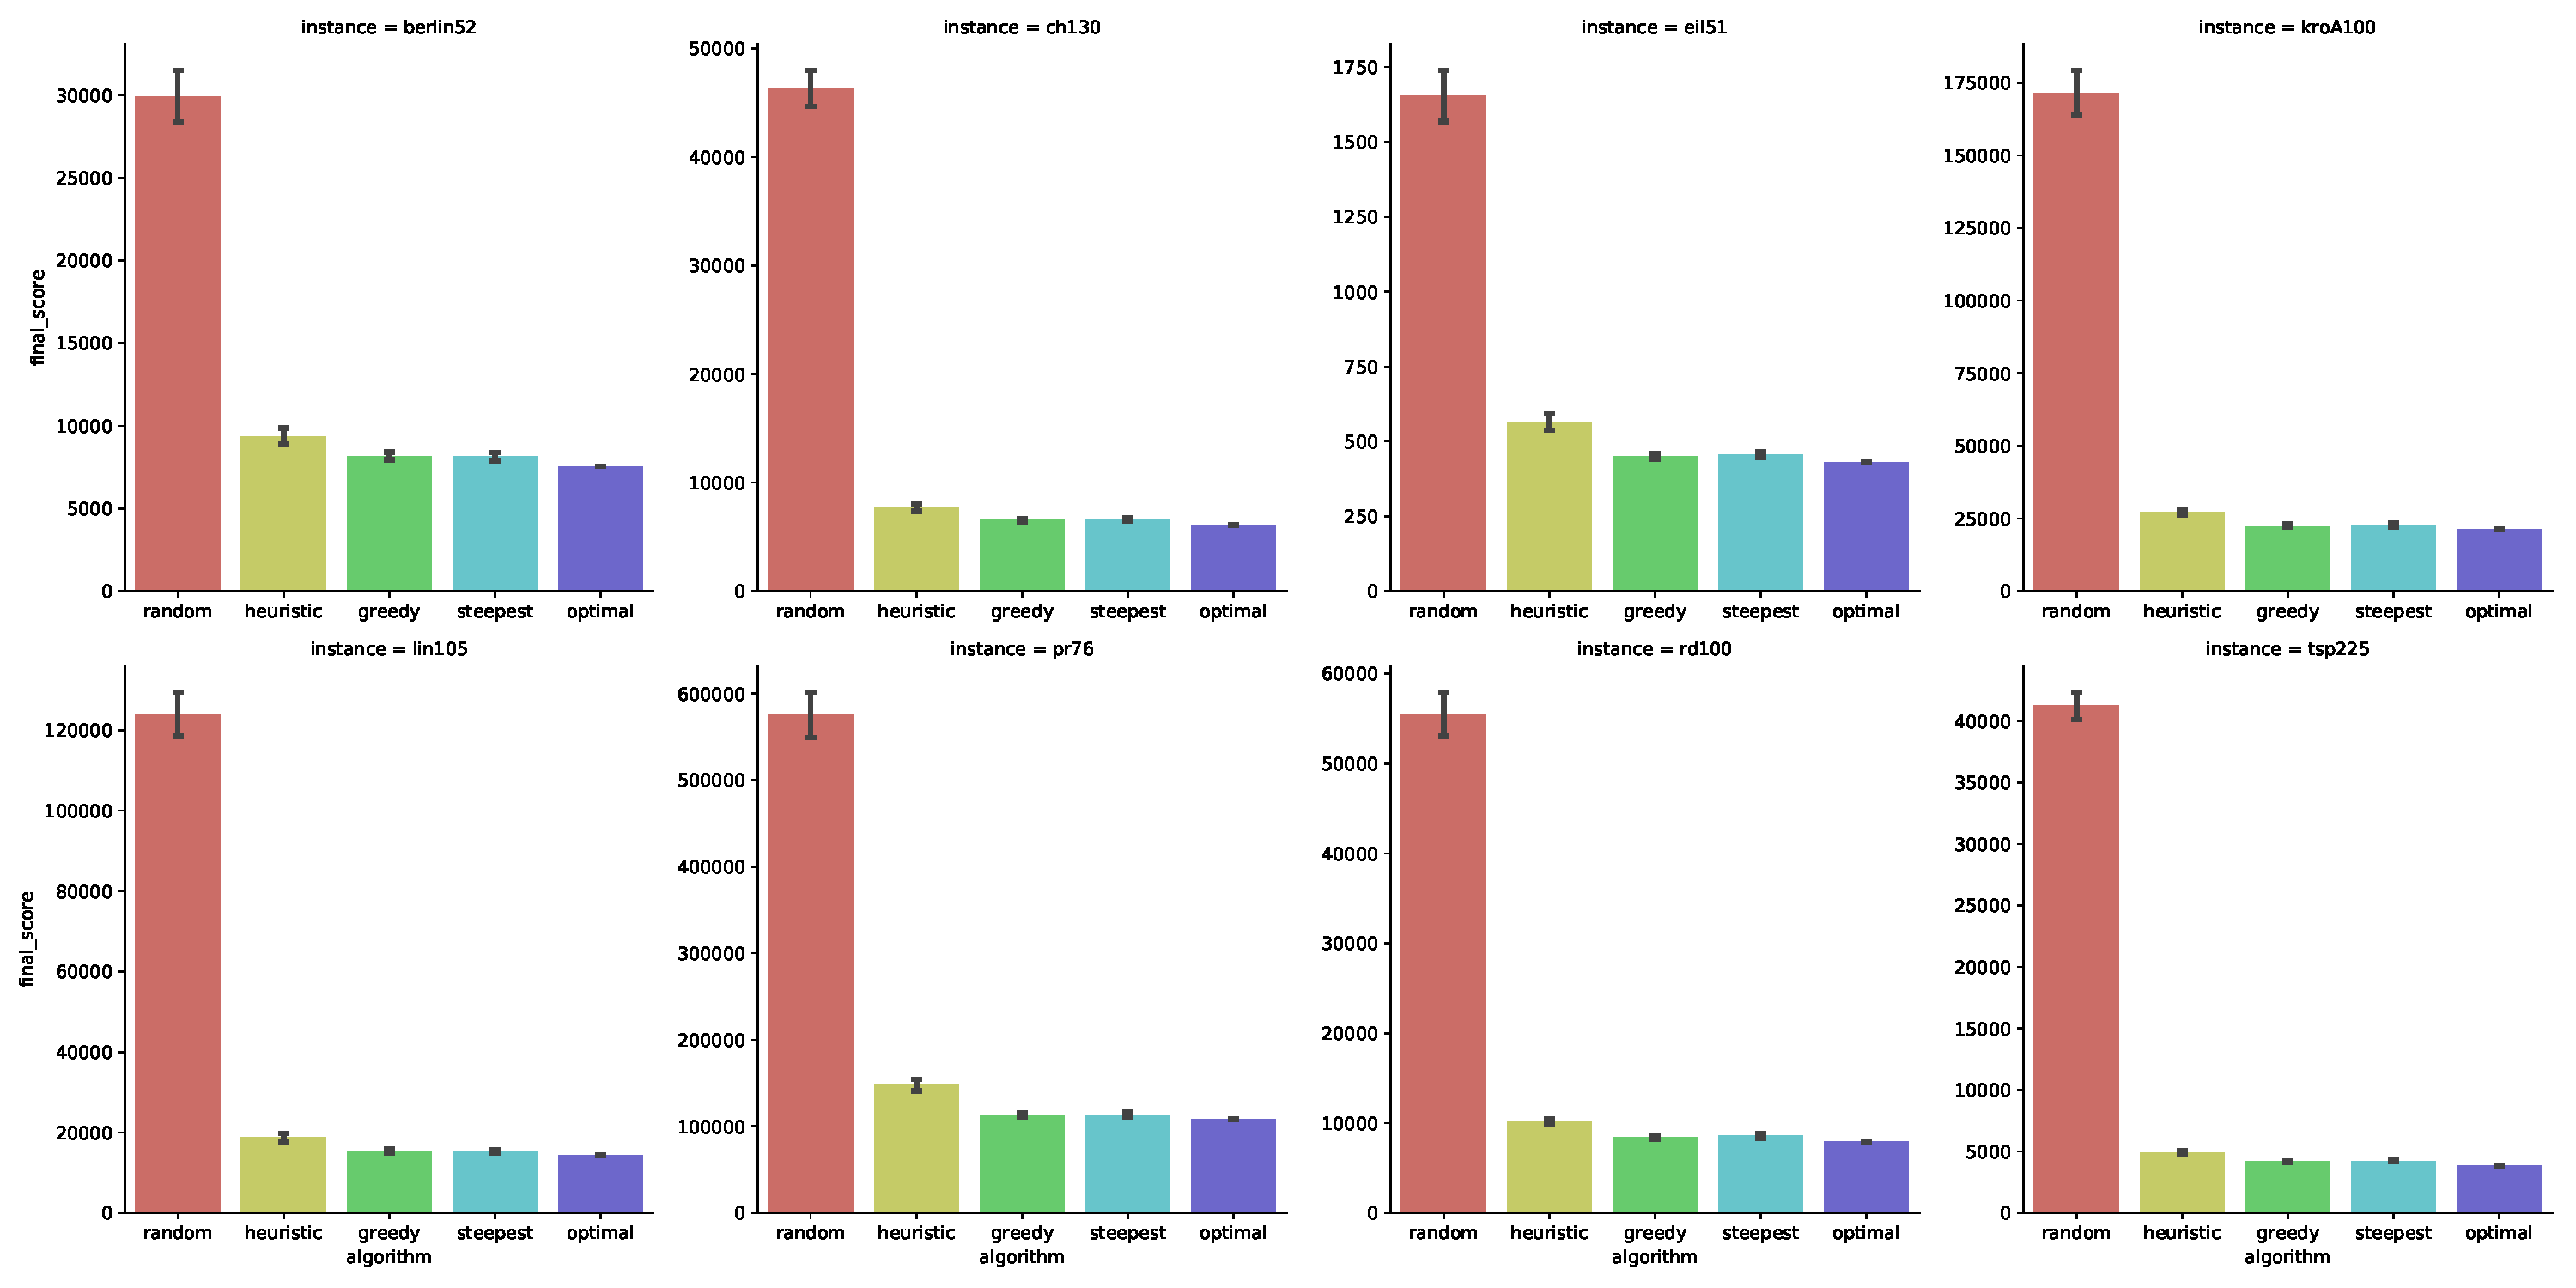
\includegraphics[width=1.0\textwidth]{graphs/score_comparison_bar_avg.pdf}
\end{center}
\caption{Porównanie średnich rozwiązań na~różnych instancjach.}
\label{fig:avg}
\end{figure}

%\begin{table}[H]
%\centering
%\begin{tabular}{ccc}%
%\hline
%\bfseries algorithm & \bfseries instance & \bfseries finalscore% specify table head
%\\ \hline
%\csvreader[head to column names]{graphs/score_comparison_bar_avg.csv}{}% use head of csv as column names
%{\\ \algorithm & \instance & \finalscore}% specify your coloumns here
%\\ \hline
%\end{tabular}
%\caption{Porównanie średnich rozwiązań na~różnych instancjach.}
%\label{tab:avg}
%\end{table}

\begin{figure}[H]
\begin{center}
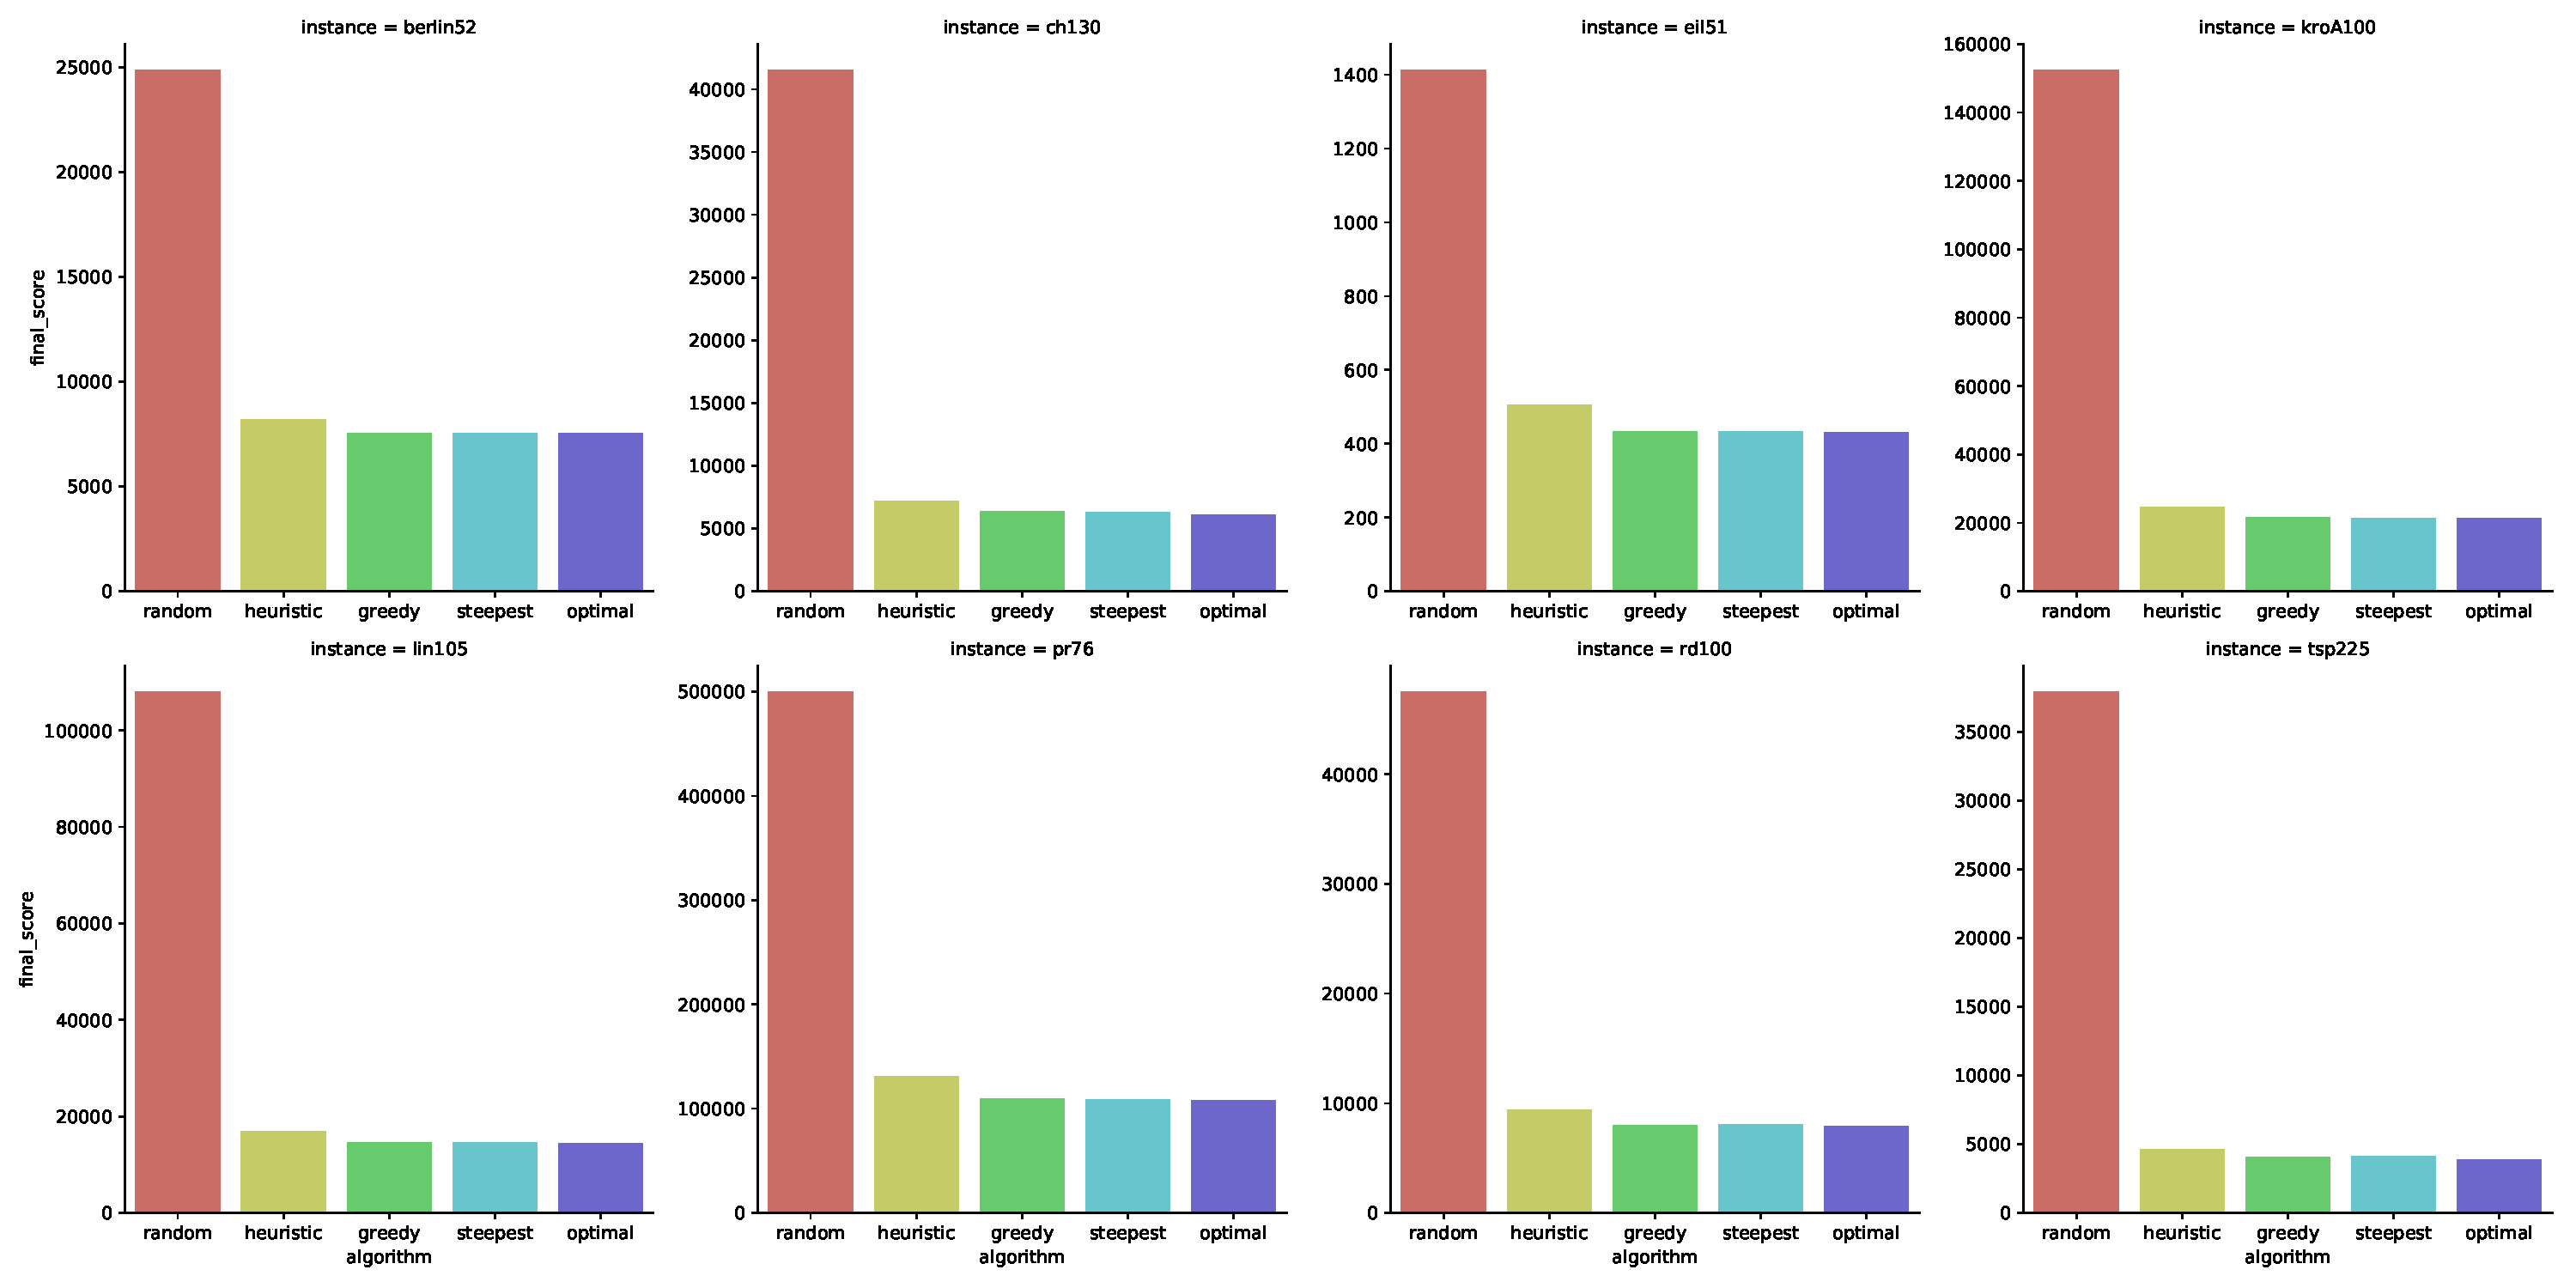
\includegraphics[width=1.0\textwidth]{graphs/score_comparison_bar_min.pdf}
\end{center}
\caption{Porównanie najlepszych znalezionych rozwiązań przez~algorytmy na~różnych instancjach.}
\label{fig:best}
\end{figure}

\begin{figure}[H]
\begin{center}
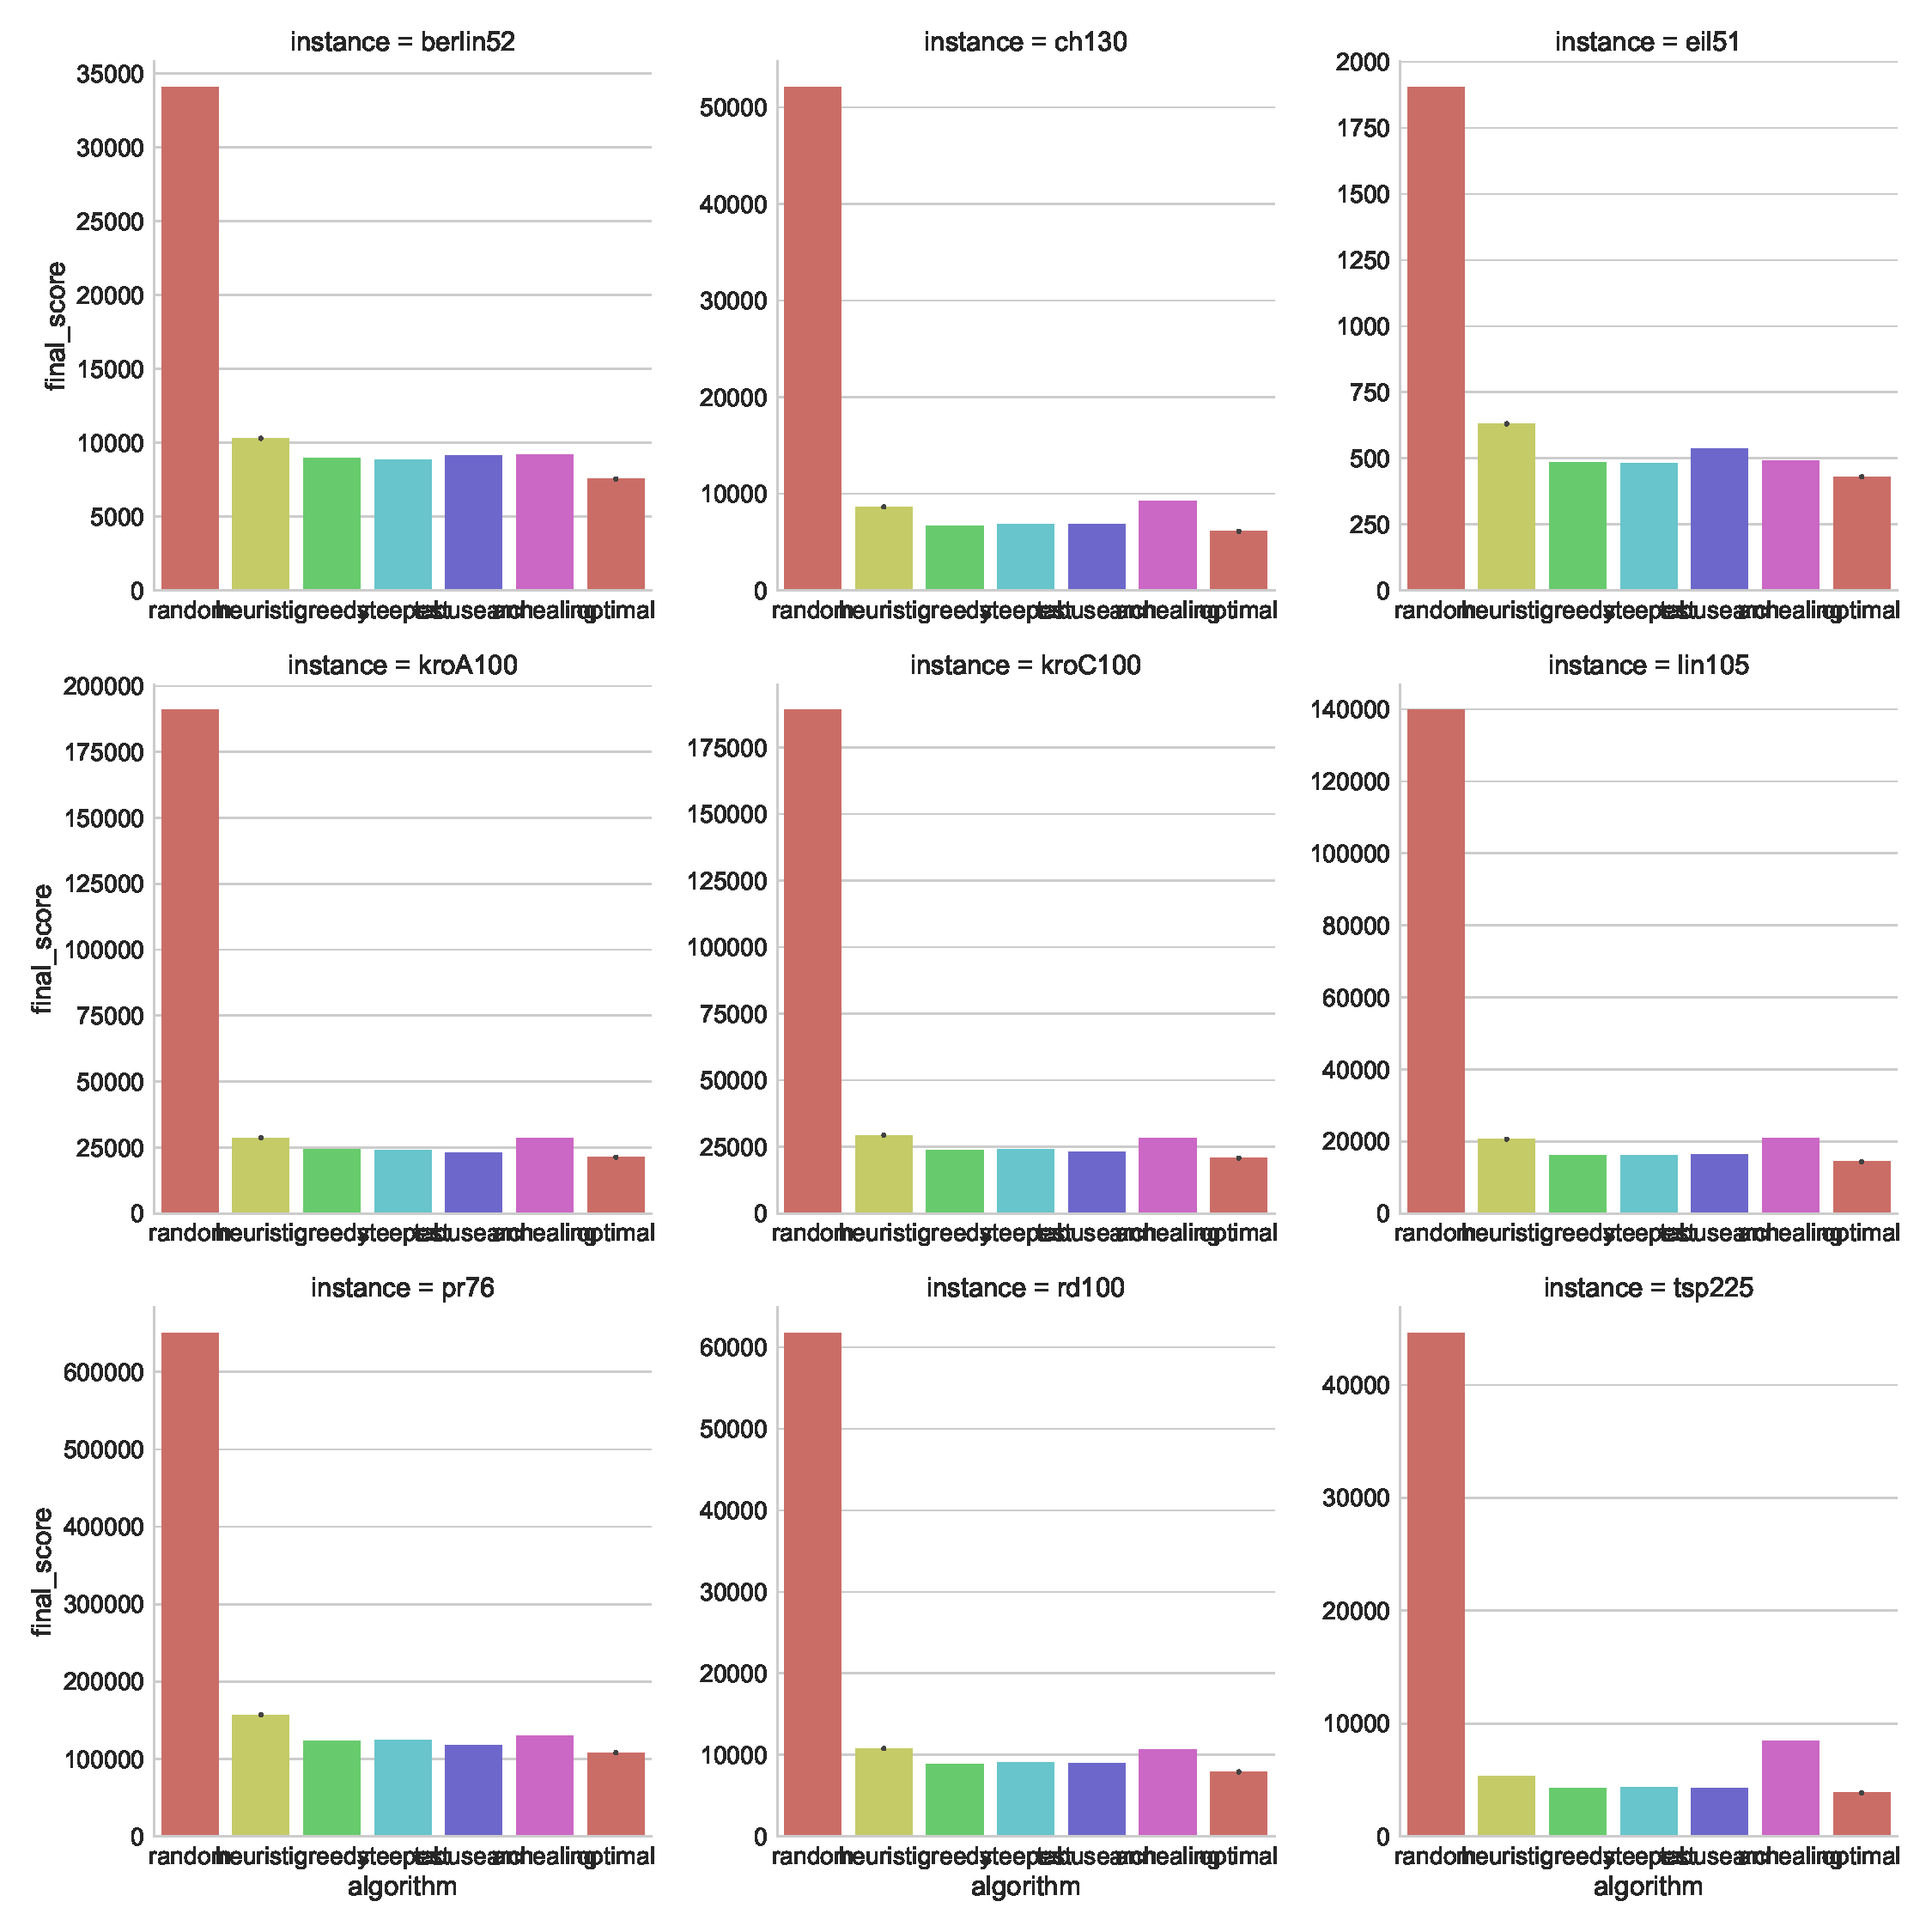
\includegraphics[width=1.0\textwidth]{graphs/score_comparison_bar_max.pdf}
\end{center}
\caption{Porównanie najgorszych znalezionych rozwiązań przez~algorytmy na~różnych instancjach.}
\label{fig:worst}
\end{figure}

\begin{figure}[H]
\begin{center}
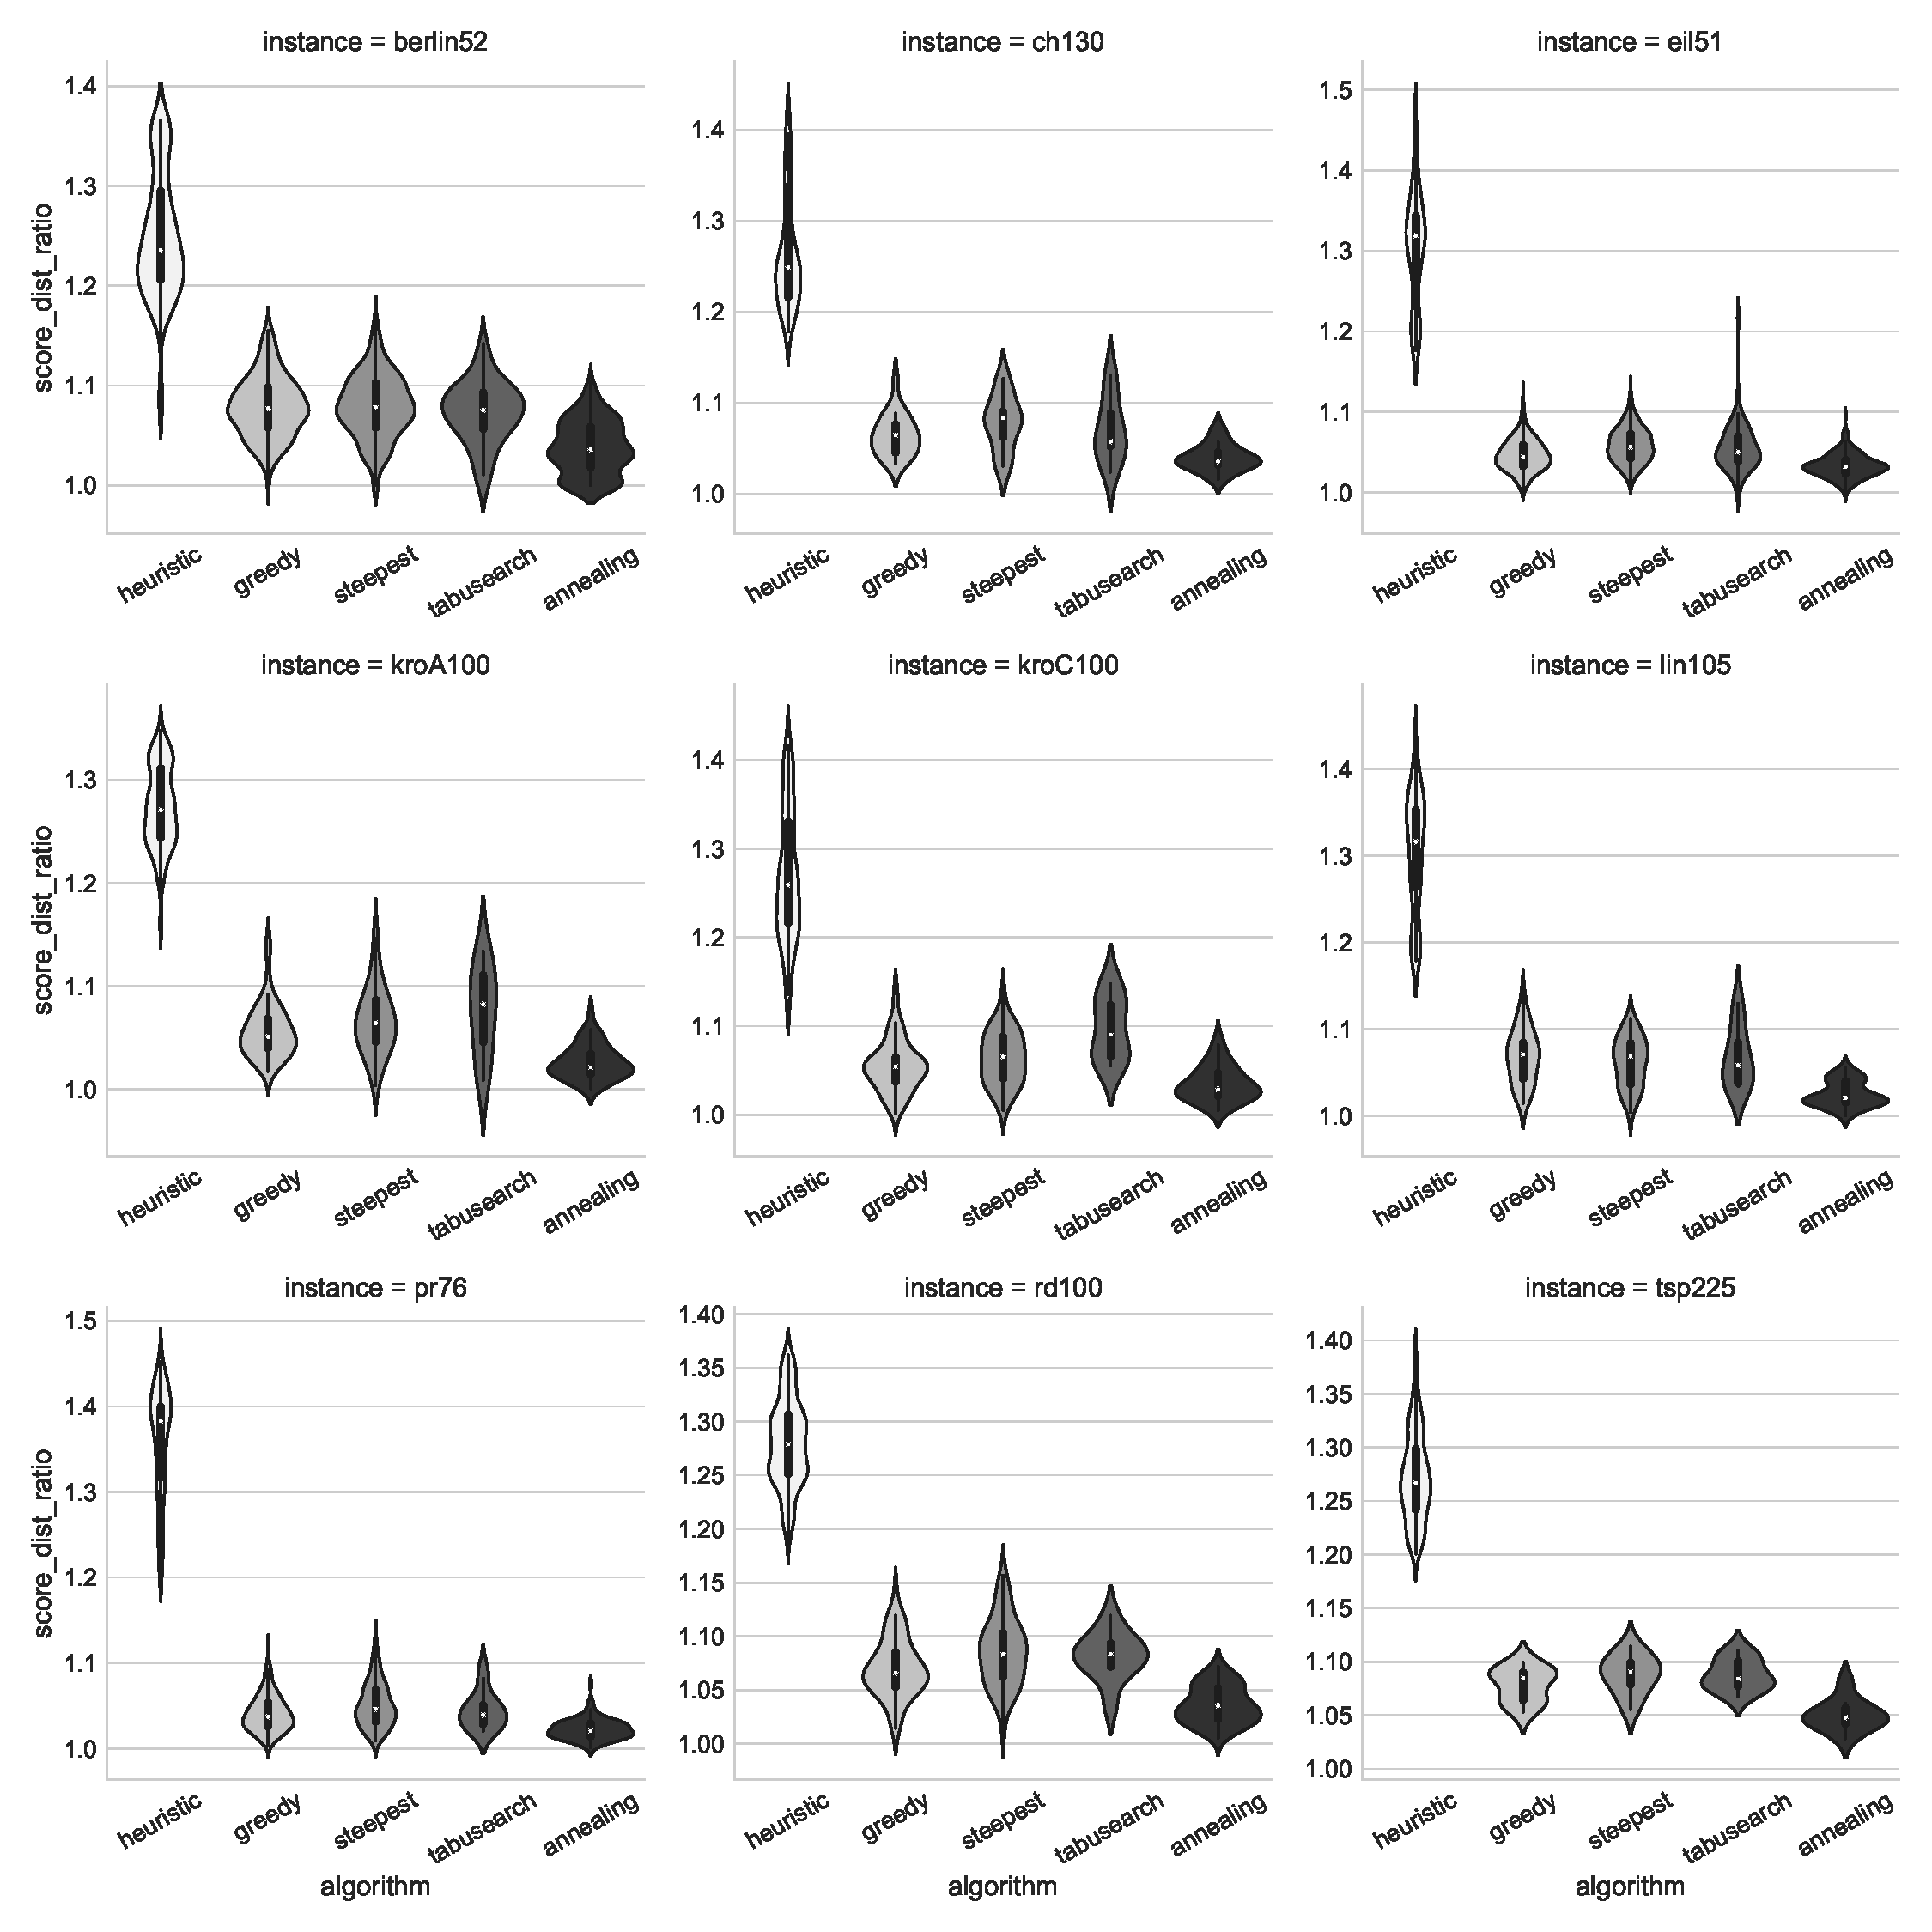
\includegraphics[width=1.0\textwidth]{graphs/score_comparison_violin.pdf}
\end{center}
\caption{Porównanie rozkładów znalezionych rozwiązań przez~algorytmy na~różnych instancjach.}
\label{fig:distribution}
\end{figure}

\subsection{Czas działania}

Heurystyka jest~zdecydowanie najszybsza, ponieważ sprawdza tylko jedno rozwiązanie. Greedy i~Steepest przeszukują przestrzeń rozwiązań, dopóki nie~mogą już~bardziej poprawić wyniku, przez co~trwają zdecydowanie najdłużej. Przeważnie obliczenia Steepesta zajmują więcej czasu, niż~wykonanie algorytmu Greedy. Na~rys.~\ref{fig:time} można~też~zauważyć, że~pojedyncze wykonania trwają znacznie dłużej od~pozostałych -- szczególnie jest~to~widoczne przy~instancji berlin52. Algorytm losowy zawsze sprawdza określoną liczbę rozwiązań, więc~czas jego działania jest~stały.

{\color{part2}
Algorytm Tabusearch trwa zdecydowanie najdłużej ze wszystkich. Jest to spowodowane dość łagodnym warunkiem stopu, przez co przeszukuje bardzo dużą przestrzeń rozwiązań -- stosunkowo większą niż pozostałe algorytmy optymalizacyjne, co widać na Rys. \ref{fig:nsol}.

Metoda symulowanego wyżarzania okazuje się zbiegać do rozwiązania finalnego w relatywnie krótkim czasie, często bliskim algorytmom przeszukiwania lokalnego. Może być to spowodowane faktem, że w początkowych iteracjach znalezienie lepszego rozwiązania lub spełnienie warunku probabilistycznego jest często spotykane, co pozytywnie wpływa na zbieżność do finalnego rozwiązania. Aczkolwiek należy zauważyć, że czas przetwarzania jest ściśle zależny od przyjętych parametrów, gdzie w przypadku przyjęcia niskiej wartości temperatury końcowej, mniejszego kroku chłodzenia, lub większej liczby iteracji bez zmiany temperatury czas przetwarzania mógłby wzrosnąć, generując jednocześnie potencjalnie lepsze rozwiązania.
}

\begin{figure}[H]
\begin{center}
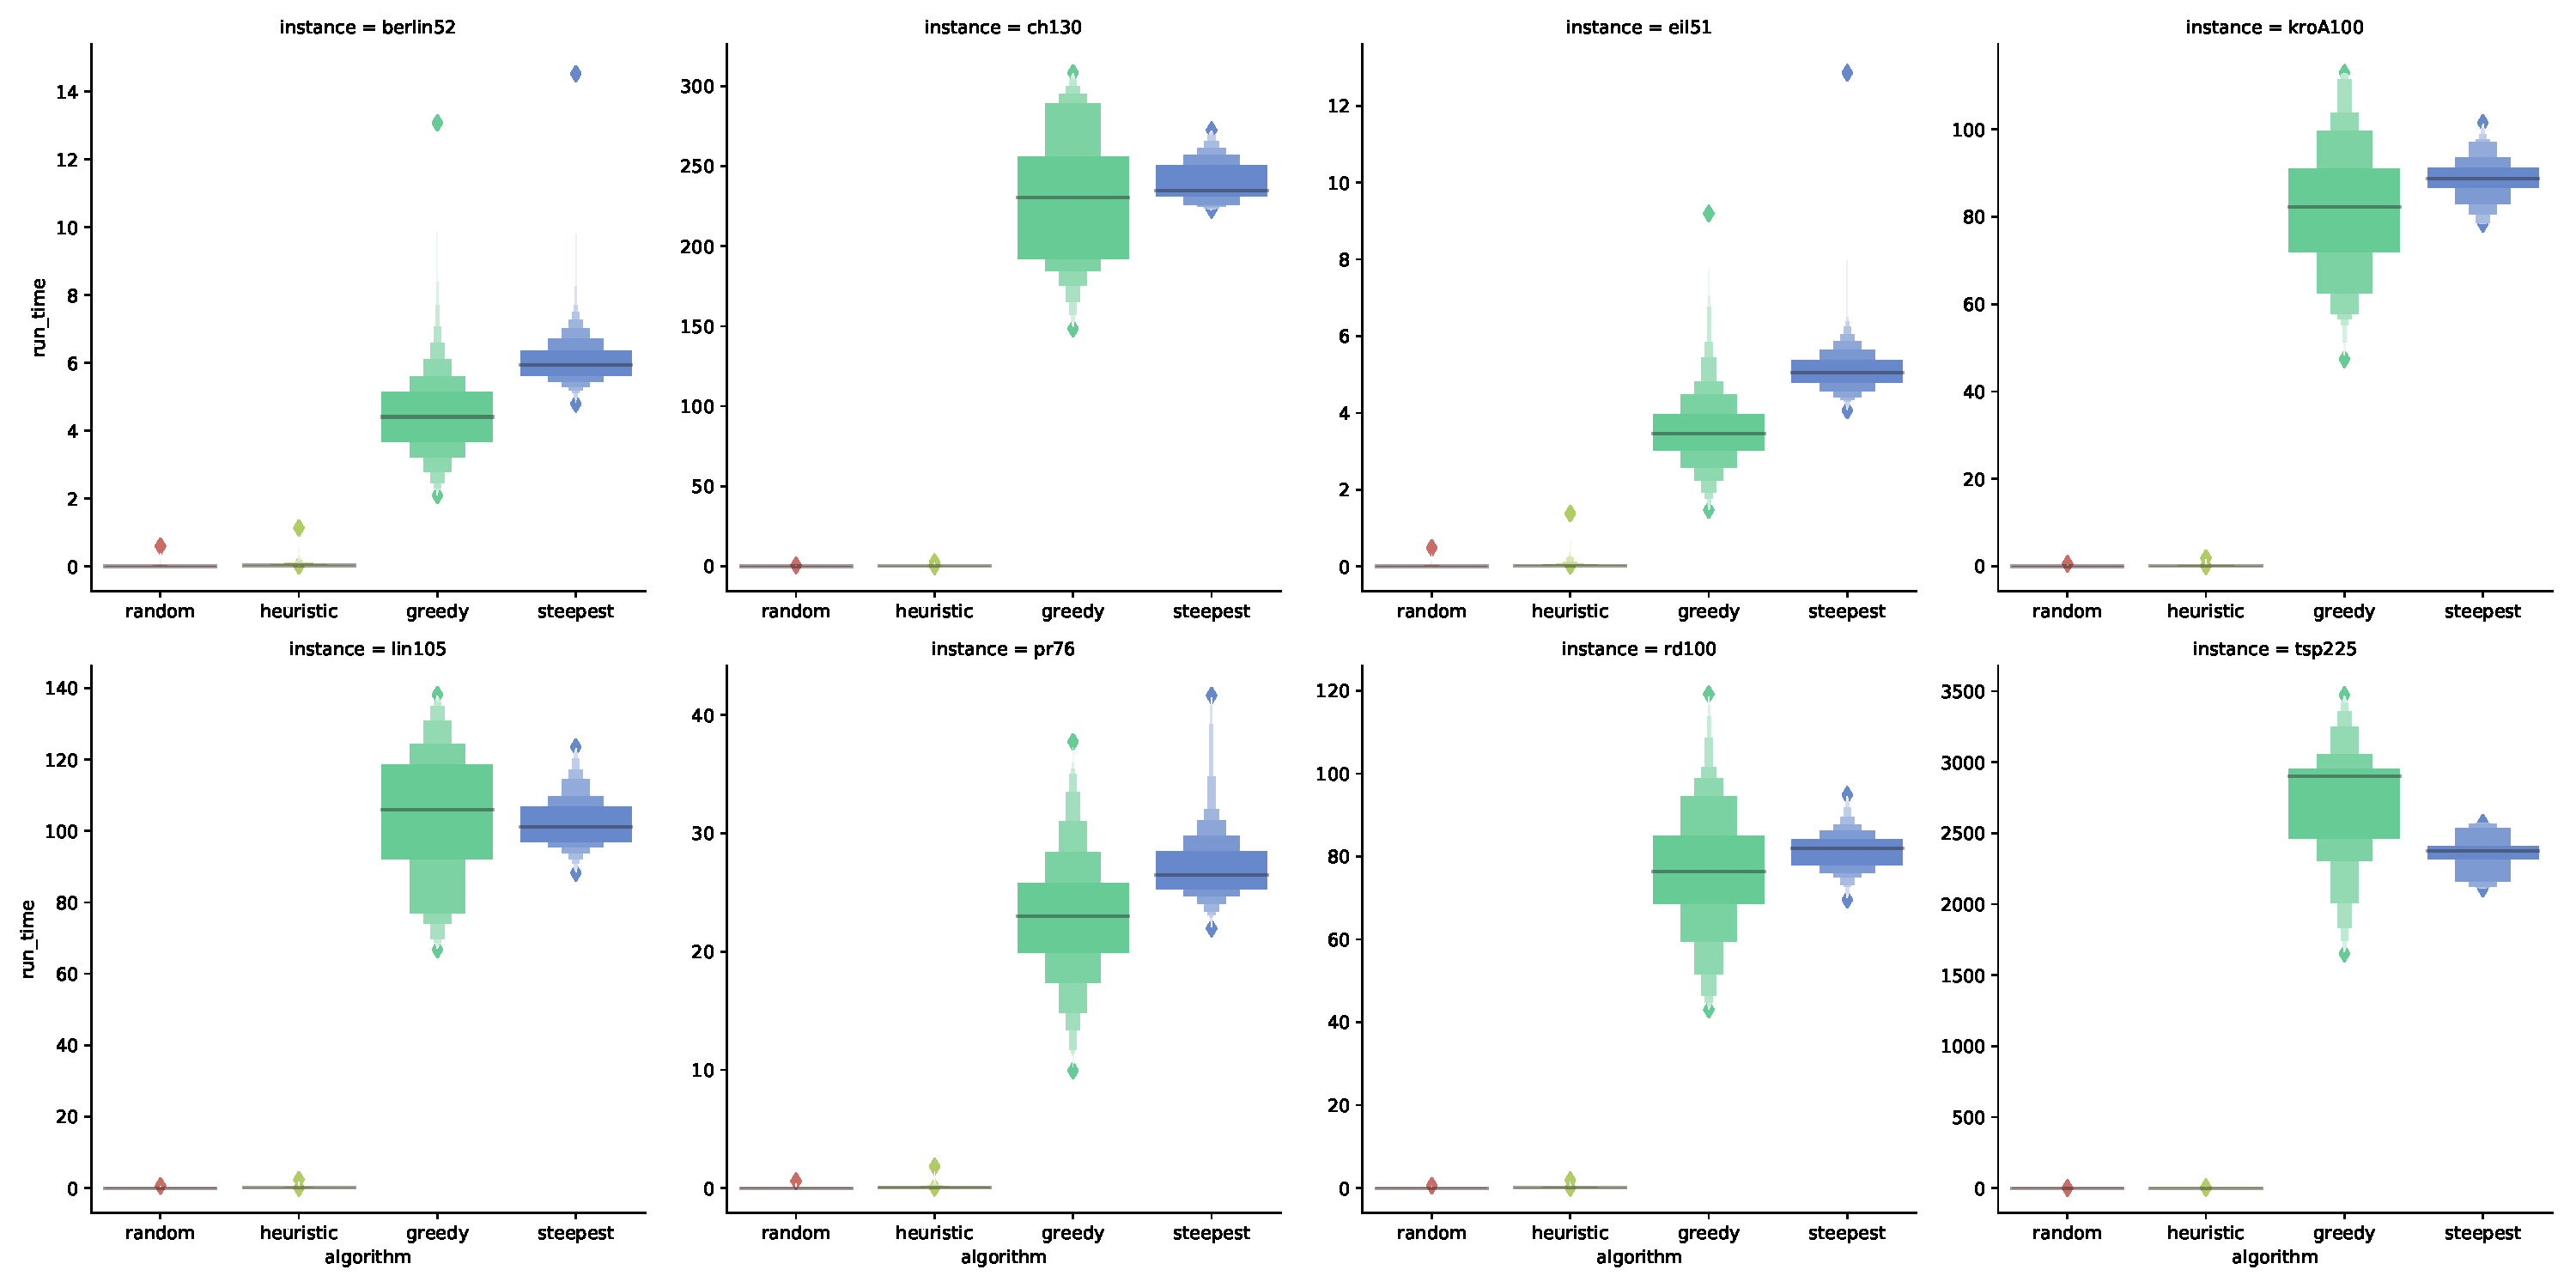
\includegraphics[width=1.0\textwidth]{graphs/time_comparison_letval.pdf}
\end{center}
\caption{Porównanie czasu działania algorytmów na~poszczególnych instancjach.}
\label{fig:time}
\end{figure}

\subsection{Efektywność algorytmów}

\subsubsection{Wybrana miara}

Aby porównać algorytmy pod~względem jakości, można to~zrobić przez zdefiniowanie kosztu czasowego, jaki~trzeba ponieść, aby~uzyskać dane rozwiązanie. Czyli należy policzyć iloraz $cost = time / result$, co~jest~przedstawione na~rys.~\ref{fig:cost}. Natomiast efektywnością algorytmu jest~odwrotność kosztu, która została przedstawiona na~rys.~\ref{fig:quality}.

\subsubsection{Wyniki}

Z~wykresów~\ref{fig:cost} i~\ref{fig:quality} można by~wyciągnąć wniosek, że~najefektywniejszym algorytmem jest~algorytm losowy, ponieważ zajmuje najmniej czasu. Takie wyniki są~jednak konsekwencją tego, że~przy każdy krok algorytmu przeszukiwania lokalnego jest~dość kosztowny, ponieważ przegląda się wiele rozwiązań, a~rozwiązanie jest~poprawiane nieznacznie (zgodnie z~założeniem algorytmów przeszukiwania lokalnego, że~funkcja celu sąsiadów niewiele się różni). Podobnie przy heurystyce -- nawet złożoność $\theta(n^2)$ nie~gwarantuje ulepszenia rozwiązania $n$-krotnie, a~jedynie kilkukrotnie, więc~koszt algorytmu jest~stosunkowo wysoki.

Na~wykresie kosztu widać również, że~Greedy jest~kosztowniejszy od~Steepesta, ponieważ daje zbliżone rozwiązania w~dłuższym czasie.

{\color{part2}
Implementacja przeszukiwania tabu okazała się najwolniejszym algorytmem ze~wszystkich badanych, w~dodatku zwracającym często minimalnie gorsze wyniki od~pozostałych, w~związku z~czym na~wykresie kosztów, wyraźnie góruje nad~innymi algorytmami.

Koszt i efektywność algorytmu symulowanego wyżarzania dla wszystkich analizowanych instancji jest zbliżony do algorytmów przeszukiwań lokalnych. Jest to związane z relatywnie krótkim czasem przetwarzania i dobrymi wynikami.

}

\begin{figure}[H]
\begin{center}
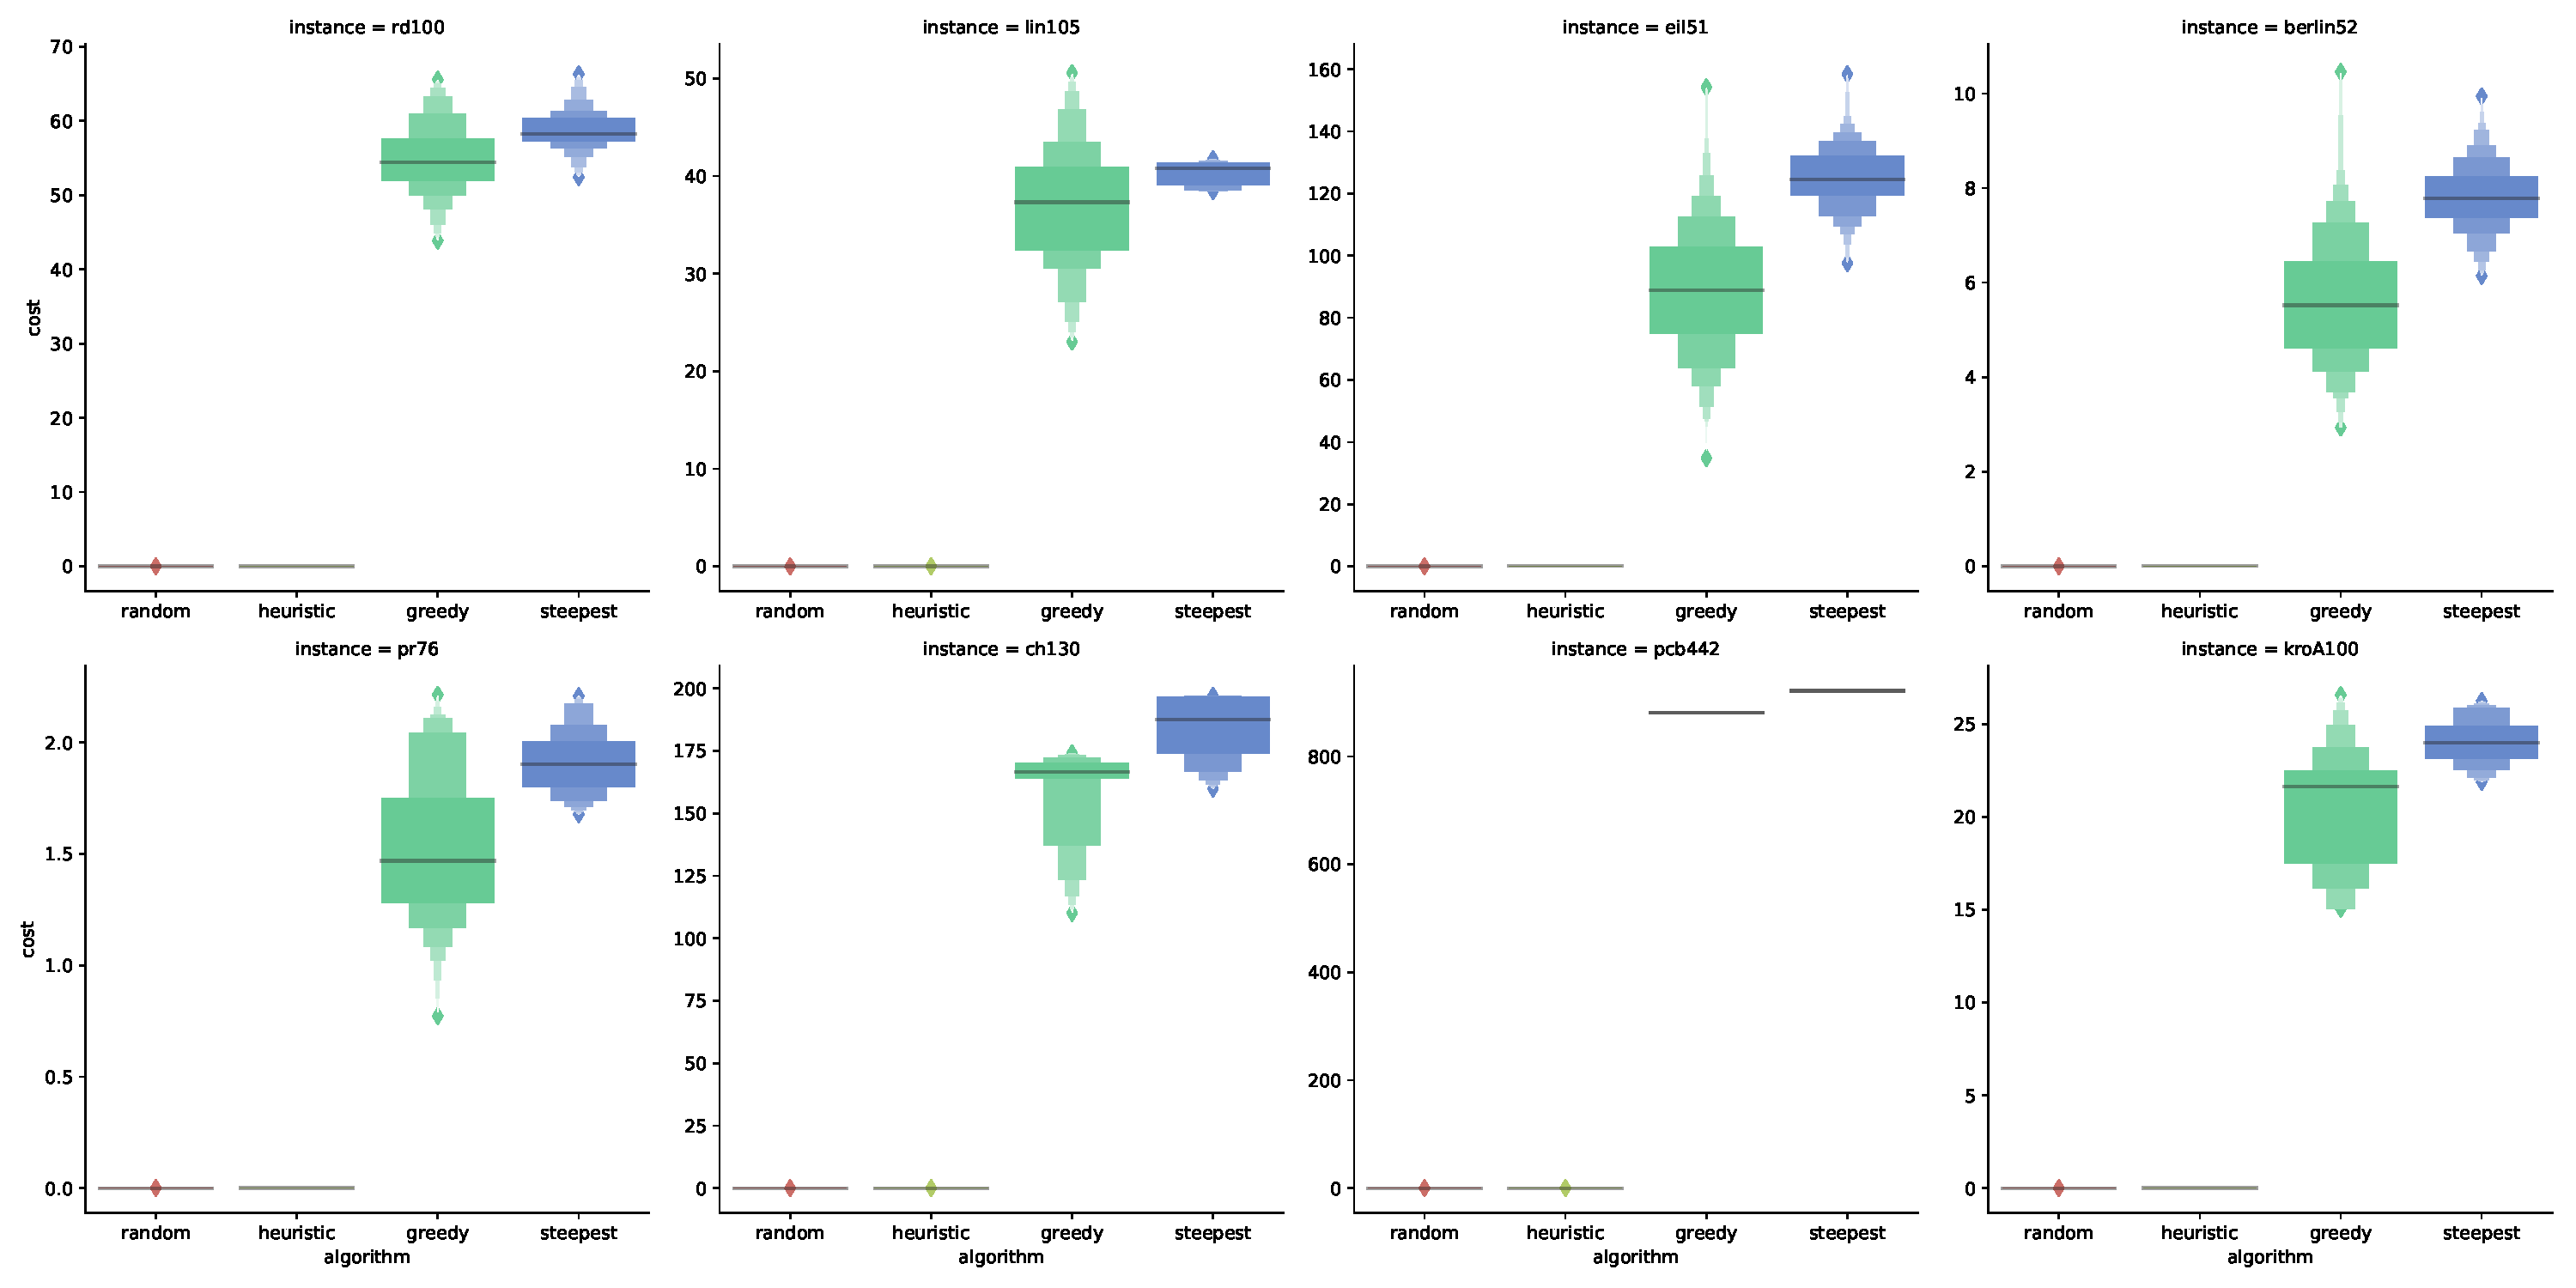
\includegraphics[width=1.0\textwidth]{graphs/cost_comparison_letval.pdf}
\end{center}
\caption{Porównanie kosztów algorytmów na~poszczególnych instancjach.}
\label{fig:cost}
\end{figure}

\begin{figure}[H]
\begin{center}
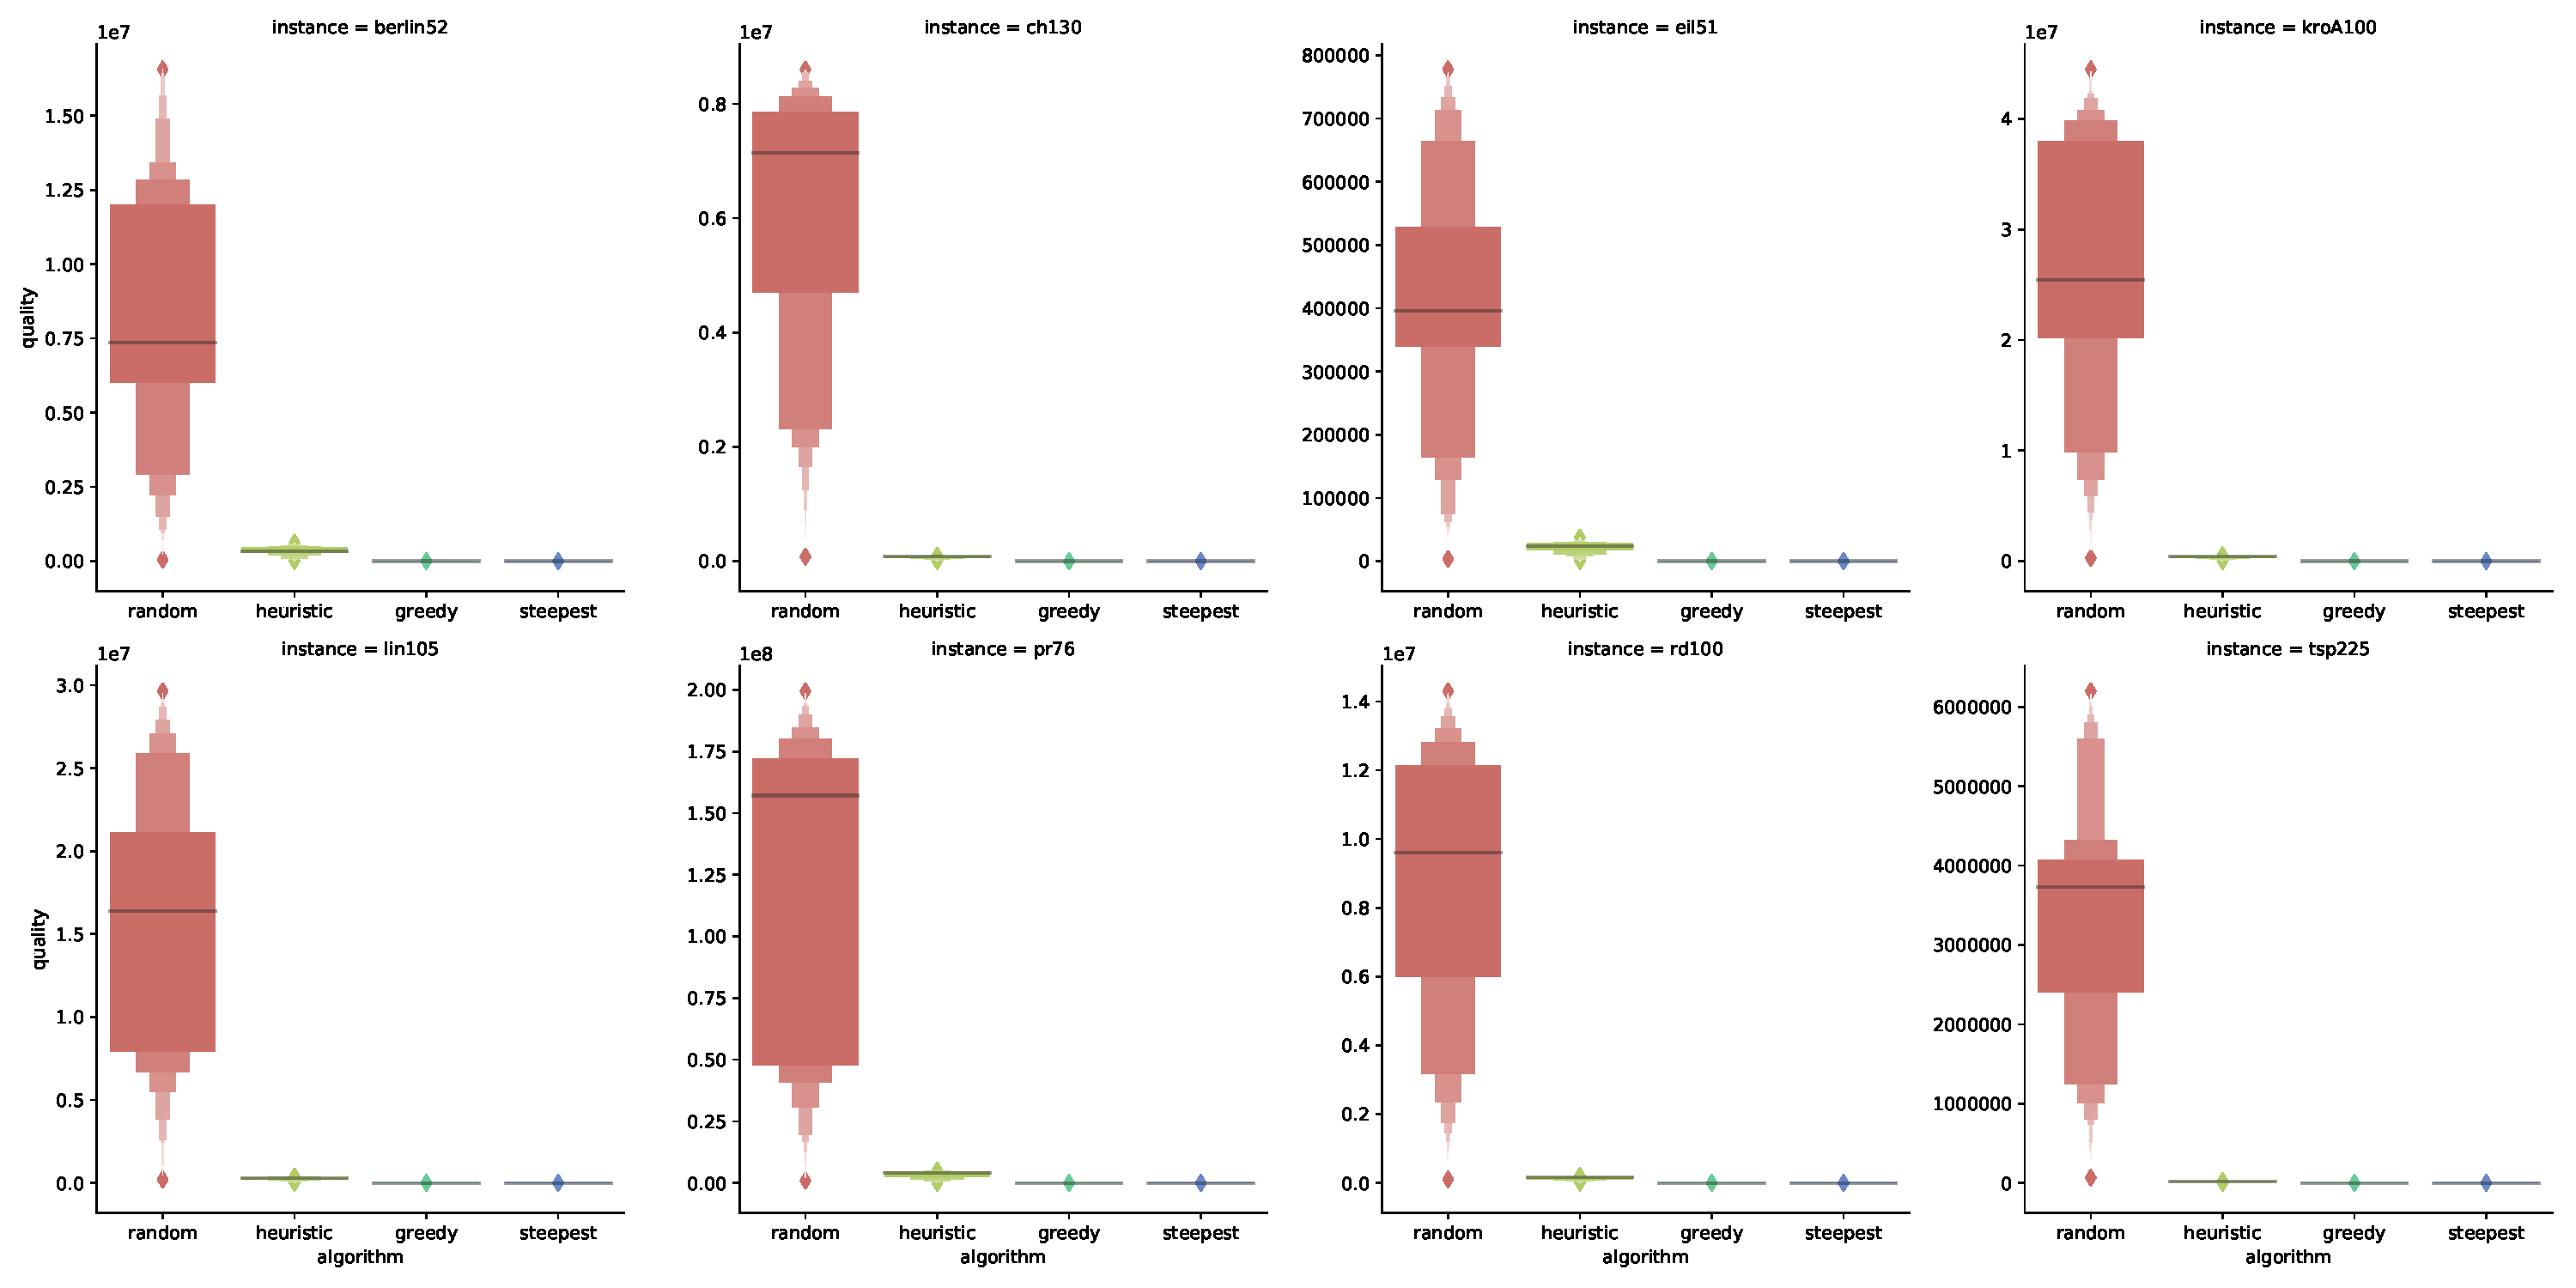
\includegraphics[width=1.0\textwidth]{graphs/quality_comparison_letval.pdf}
\end{center}
\caption{Porównanie efektywności algorytmów na~poszczególnych instancjach.}
\label{fig:quality}
\end{figure}

\subsection{Liczba kroków algorytmów lokalnego przeszukiwania}

Wykres~\ref{fig:steps} przedstawia liczbę kroków wykonanych przez algorytmy lokalnego przeszukiwania. Widać, że~Greedy wykonuje ich kilkakrotnie więcej niż~Steepest, a~także, że~liczba wykonanych kroków przez ten~algorytm jest~dużo bardziej zróżnicowana, w~zależności od~przypadku startowego. Jest~to~spowodowane tym, że~algorytm Steepest we~wcześniejszym kroku osiąga lokalnie najlepsze rozwiązanie, ponieważ za~każdym razem wybiera to, które~najbardziej poprawia wynik z~całego sąsiedztwa.

{\color{part2}
Algorytm Tabu Search wykonuje więcej kroków niż algorytmy lokalnego przeszukiwania. Nie zatrzymuje się on na optimach lokalnych, ale stara się z nich wychodzić, w poszukiwaniu lepszych rozwiązań tak długo, aż nie znajduje ulepszeń po określonej liczbie kroków.

Algorytm symulowanego wyżarzanie wykonuje wielokrotnie więcej kroków od pozostałych algorytmów, co jest spowodowane długim czasem wyżarzania i dojścia do rozwiązania finalnego. Należy pamiętać, że manipulowanie odpowiednimi parametrami mogłoby skrócić lub wydłużyć liczbę kroków.
}

\begin{figure}[H]
\begin{center}
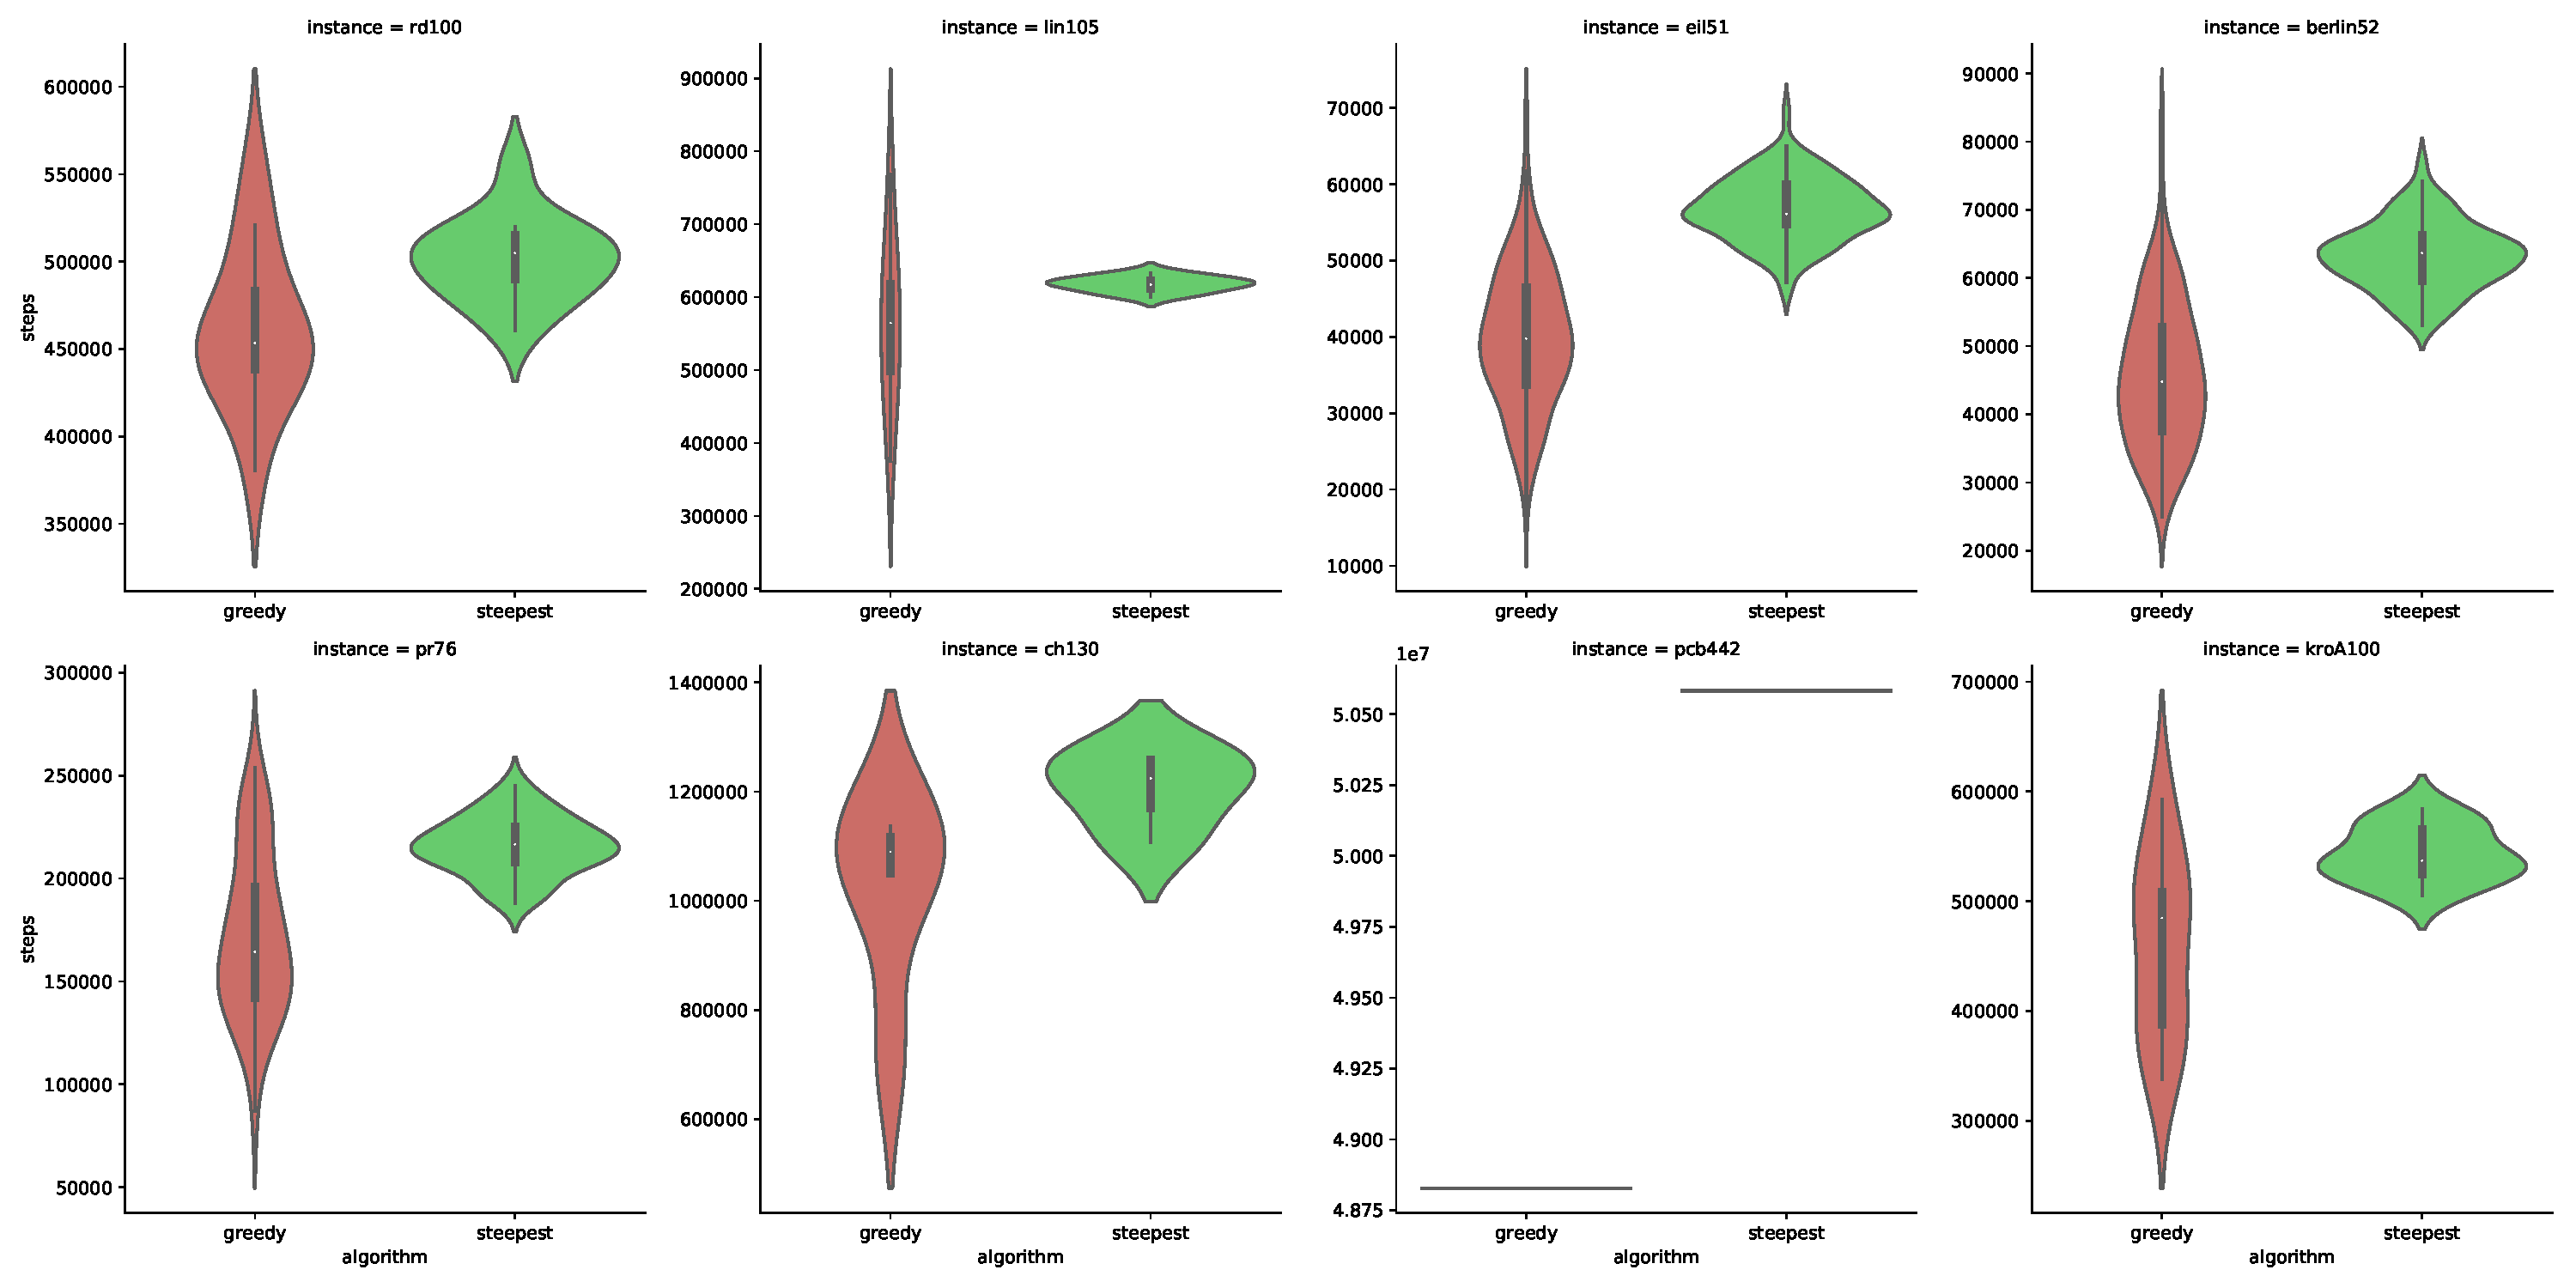
\includegraphics[width=1.0\textwidth]{graphs/steps_comparison_violin.pdf}
\end{center}
\caption{Porównanie algorytmów pod~względem liczby kroków do~zatrzymania.}
\label{fig:steps}
\end{figure}

\subsection{Średnia liczba przeszukanych rozwiązań}

Na~wykresie \ref{fig:nsol} jest~przedstawiona liczba rozwiązań przeszukiwanych przez~oba rozważane algorytmy lokalnego przeszukiwania. Można na~nim~zauważyć, że~średnio Steepest przeszukuje większą przestrzeń, choć~zdarzają się wykonania algorytmu Greedy, które~sprawdzają większą liczbę rozwiązań. Jest to~o~tyle ciekawe, że~Steepest wykonuje mniej kroków, niż~Greedy, a~i~tak aby~je~wykonać, przegląda więcej rozwiązań. Co~ciekawe, ta~tendencja jest~odmienna dla~największej instancji; podobnie~też, czas działania algorytmu Greedy dla~niej jest~większy od~Steepesta.

{\color{part2}
Przeszukiwanie tabu nie tylko wykonuje najwięcej kroków, ale też przegląda najwięcej rozwiązań.

Algorytm symulowanego wyżarzania pomimo wykonywania wielu kroków przegląda mniejszą liczbę rozwiązań, co jest związane ściśle z zastosowaną funkcją generowania losowych rozwiązań.
}

\begin{figure}[H]
\begin{center}
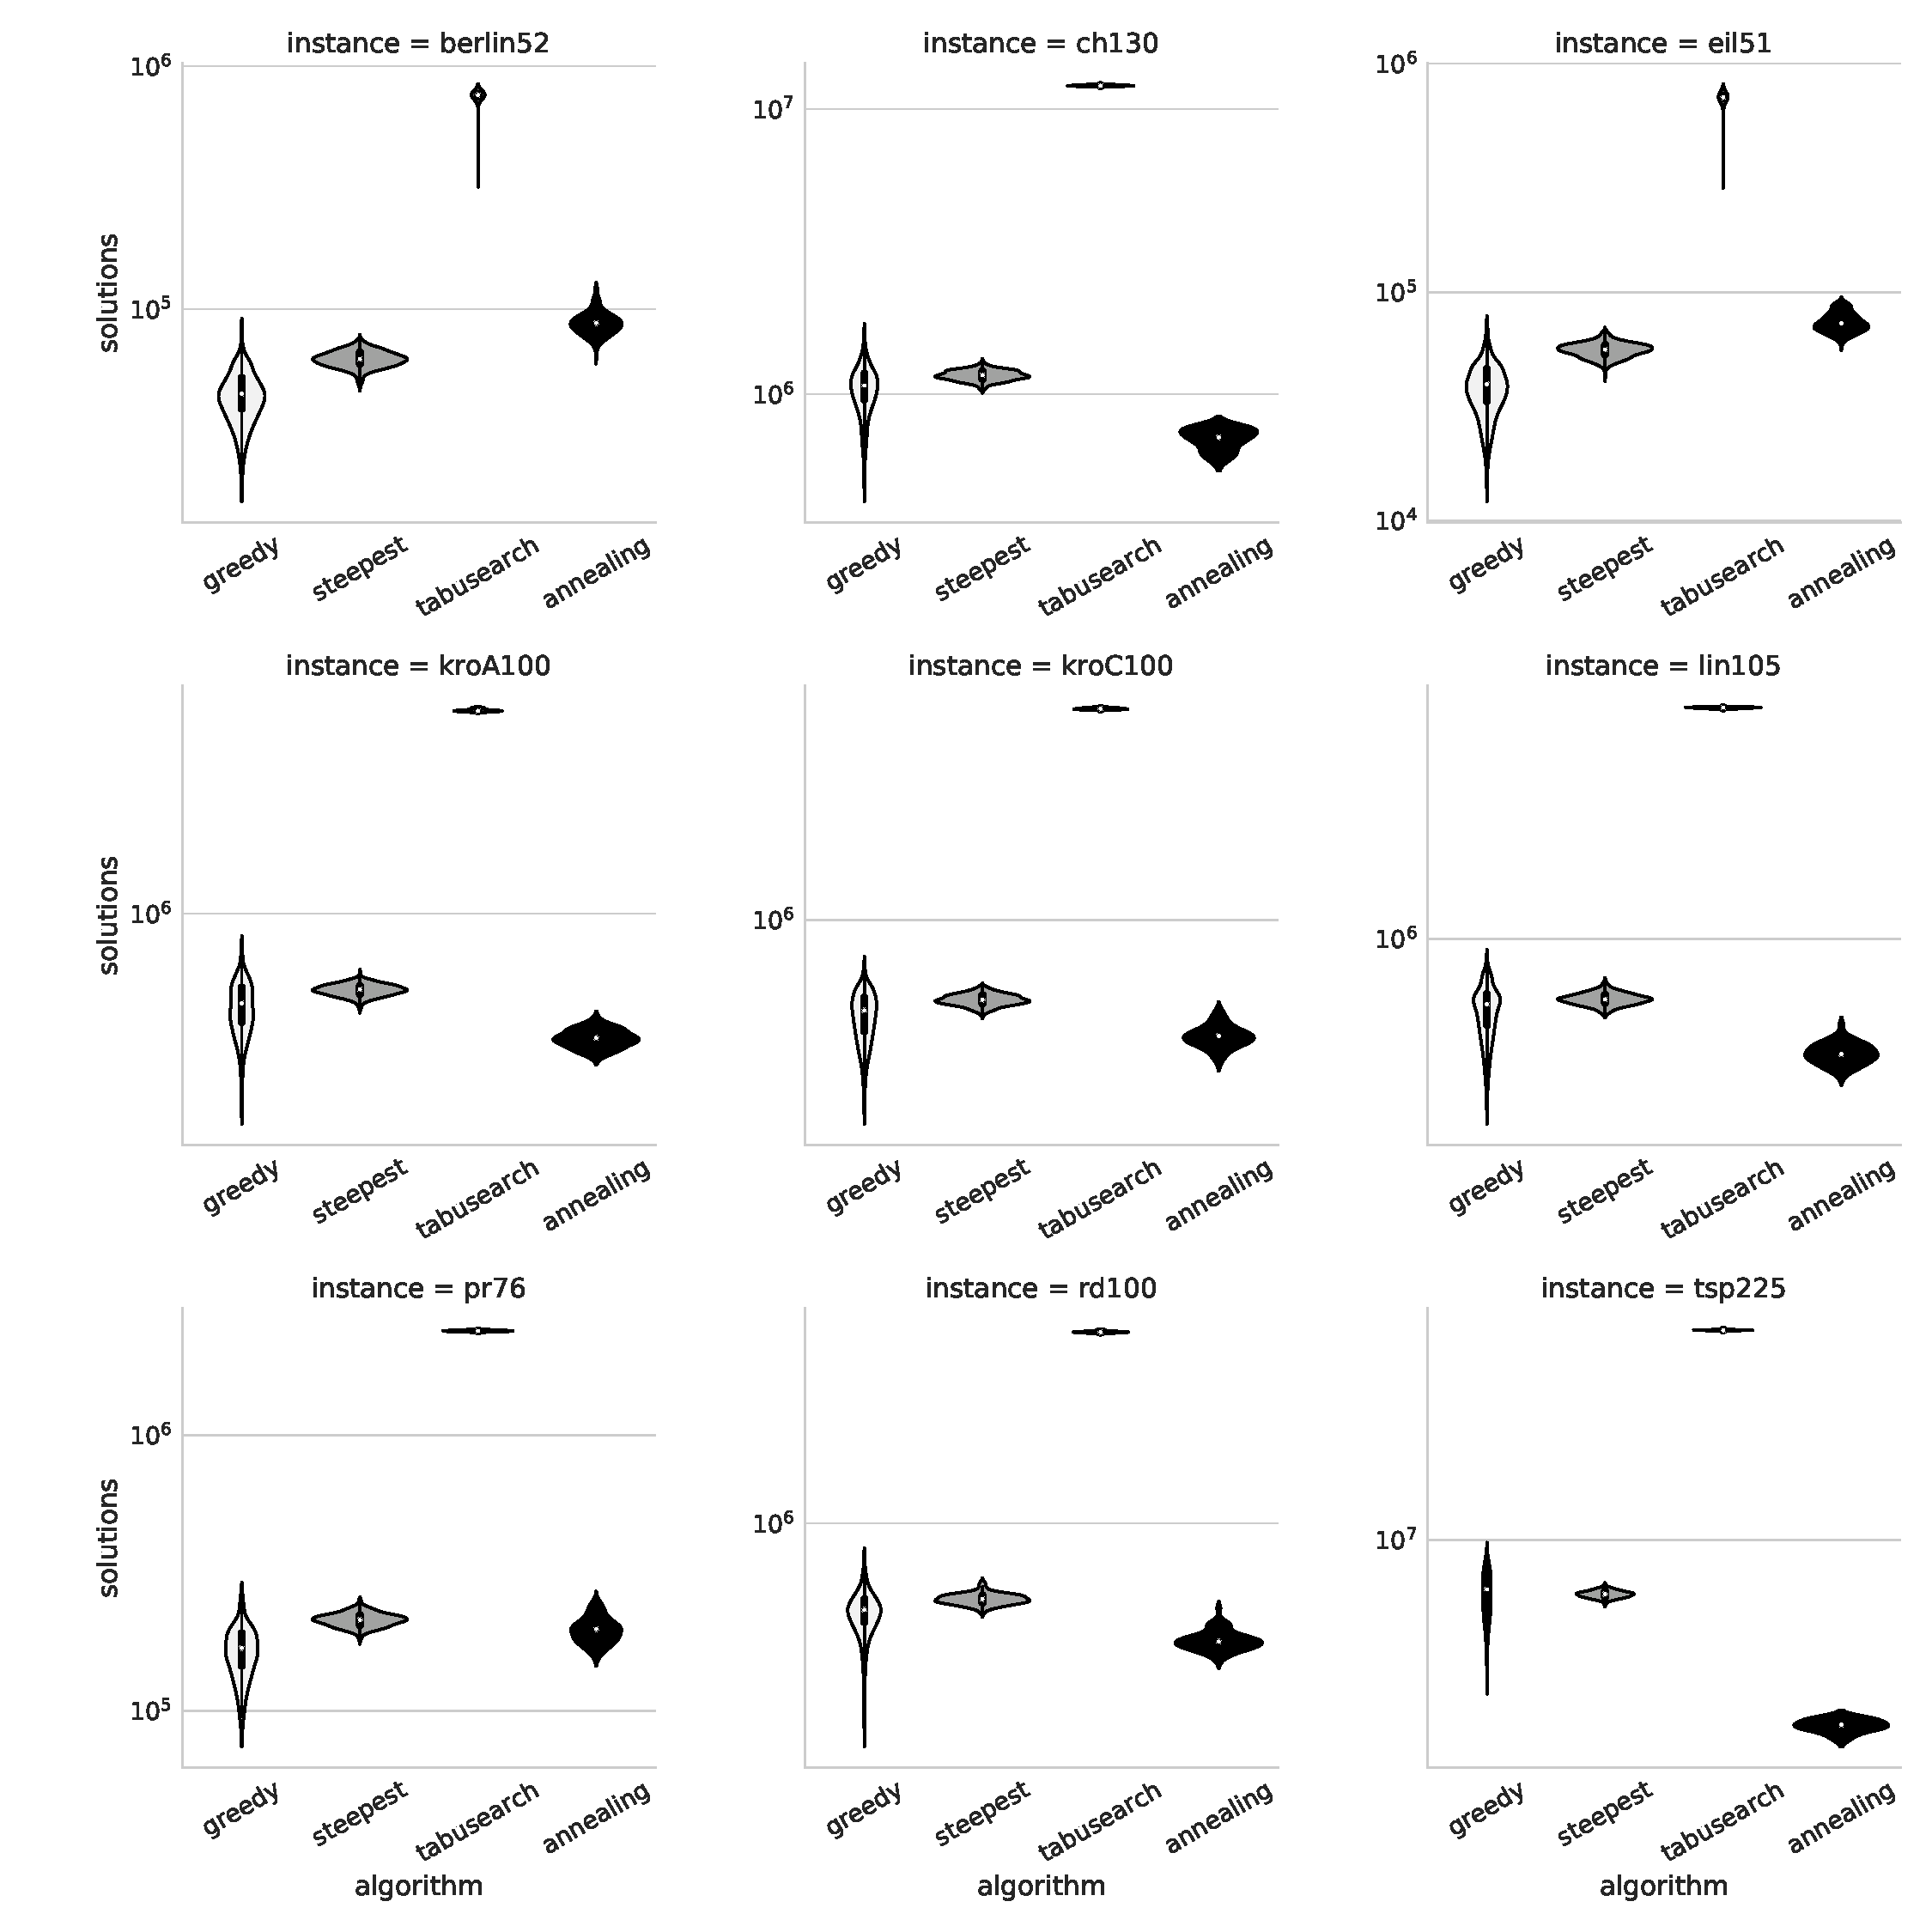
\includegraphics[width=1.0\textwidth]{graphs/solutions_comparison_violin.pdf}
\end{center}
\caption{Porównanie algorytmów pod~względem liczby przeszukanych rozwiązań.}
\label{fig:nsol}
\end{figure}

\subsection{Przeszukiwanie lokalne}

\subsubsection{Jakość rozwiązania początkowego a końcowego}

Badając zależność między rozwiązaniem początkowym, a~końcowym, nie~udało nam się zaobserwować związku na~wykresie punktowym \ref{fig:diff_point}. Punkty są~bardzo rozrzucone i~nie~daje się ich~odpowiednio pogrupować. Na~wykresie skrzypcowym~\ref{fig:diff} zostały przedstawione rozwiązania początkowe i~końcowe dla~obu~algorytmów. Widać, że~są~wyraźnie od~siebie oddalone i~zgrupowane w~osobne chmury. Można zatem przypuszczać, że~jakość rozwiązania końcowego nie~zależy od~jakości rozwiązania początkowego.

\begin{figure}[H]
\begin{center}
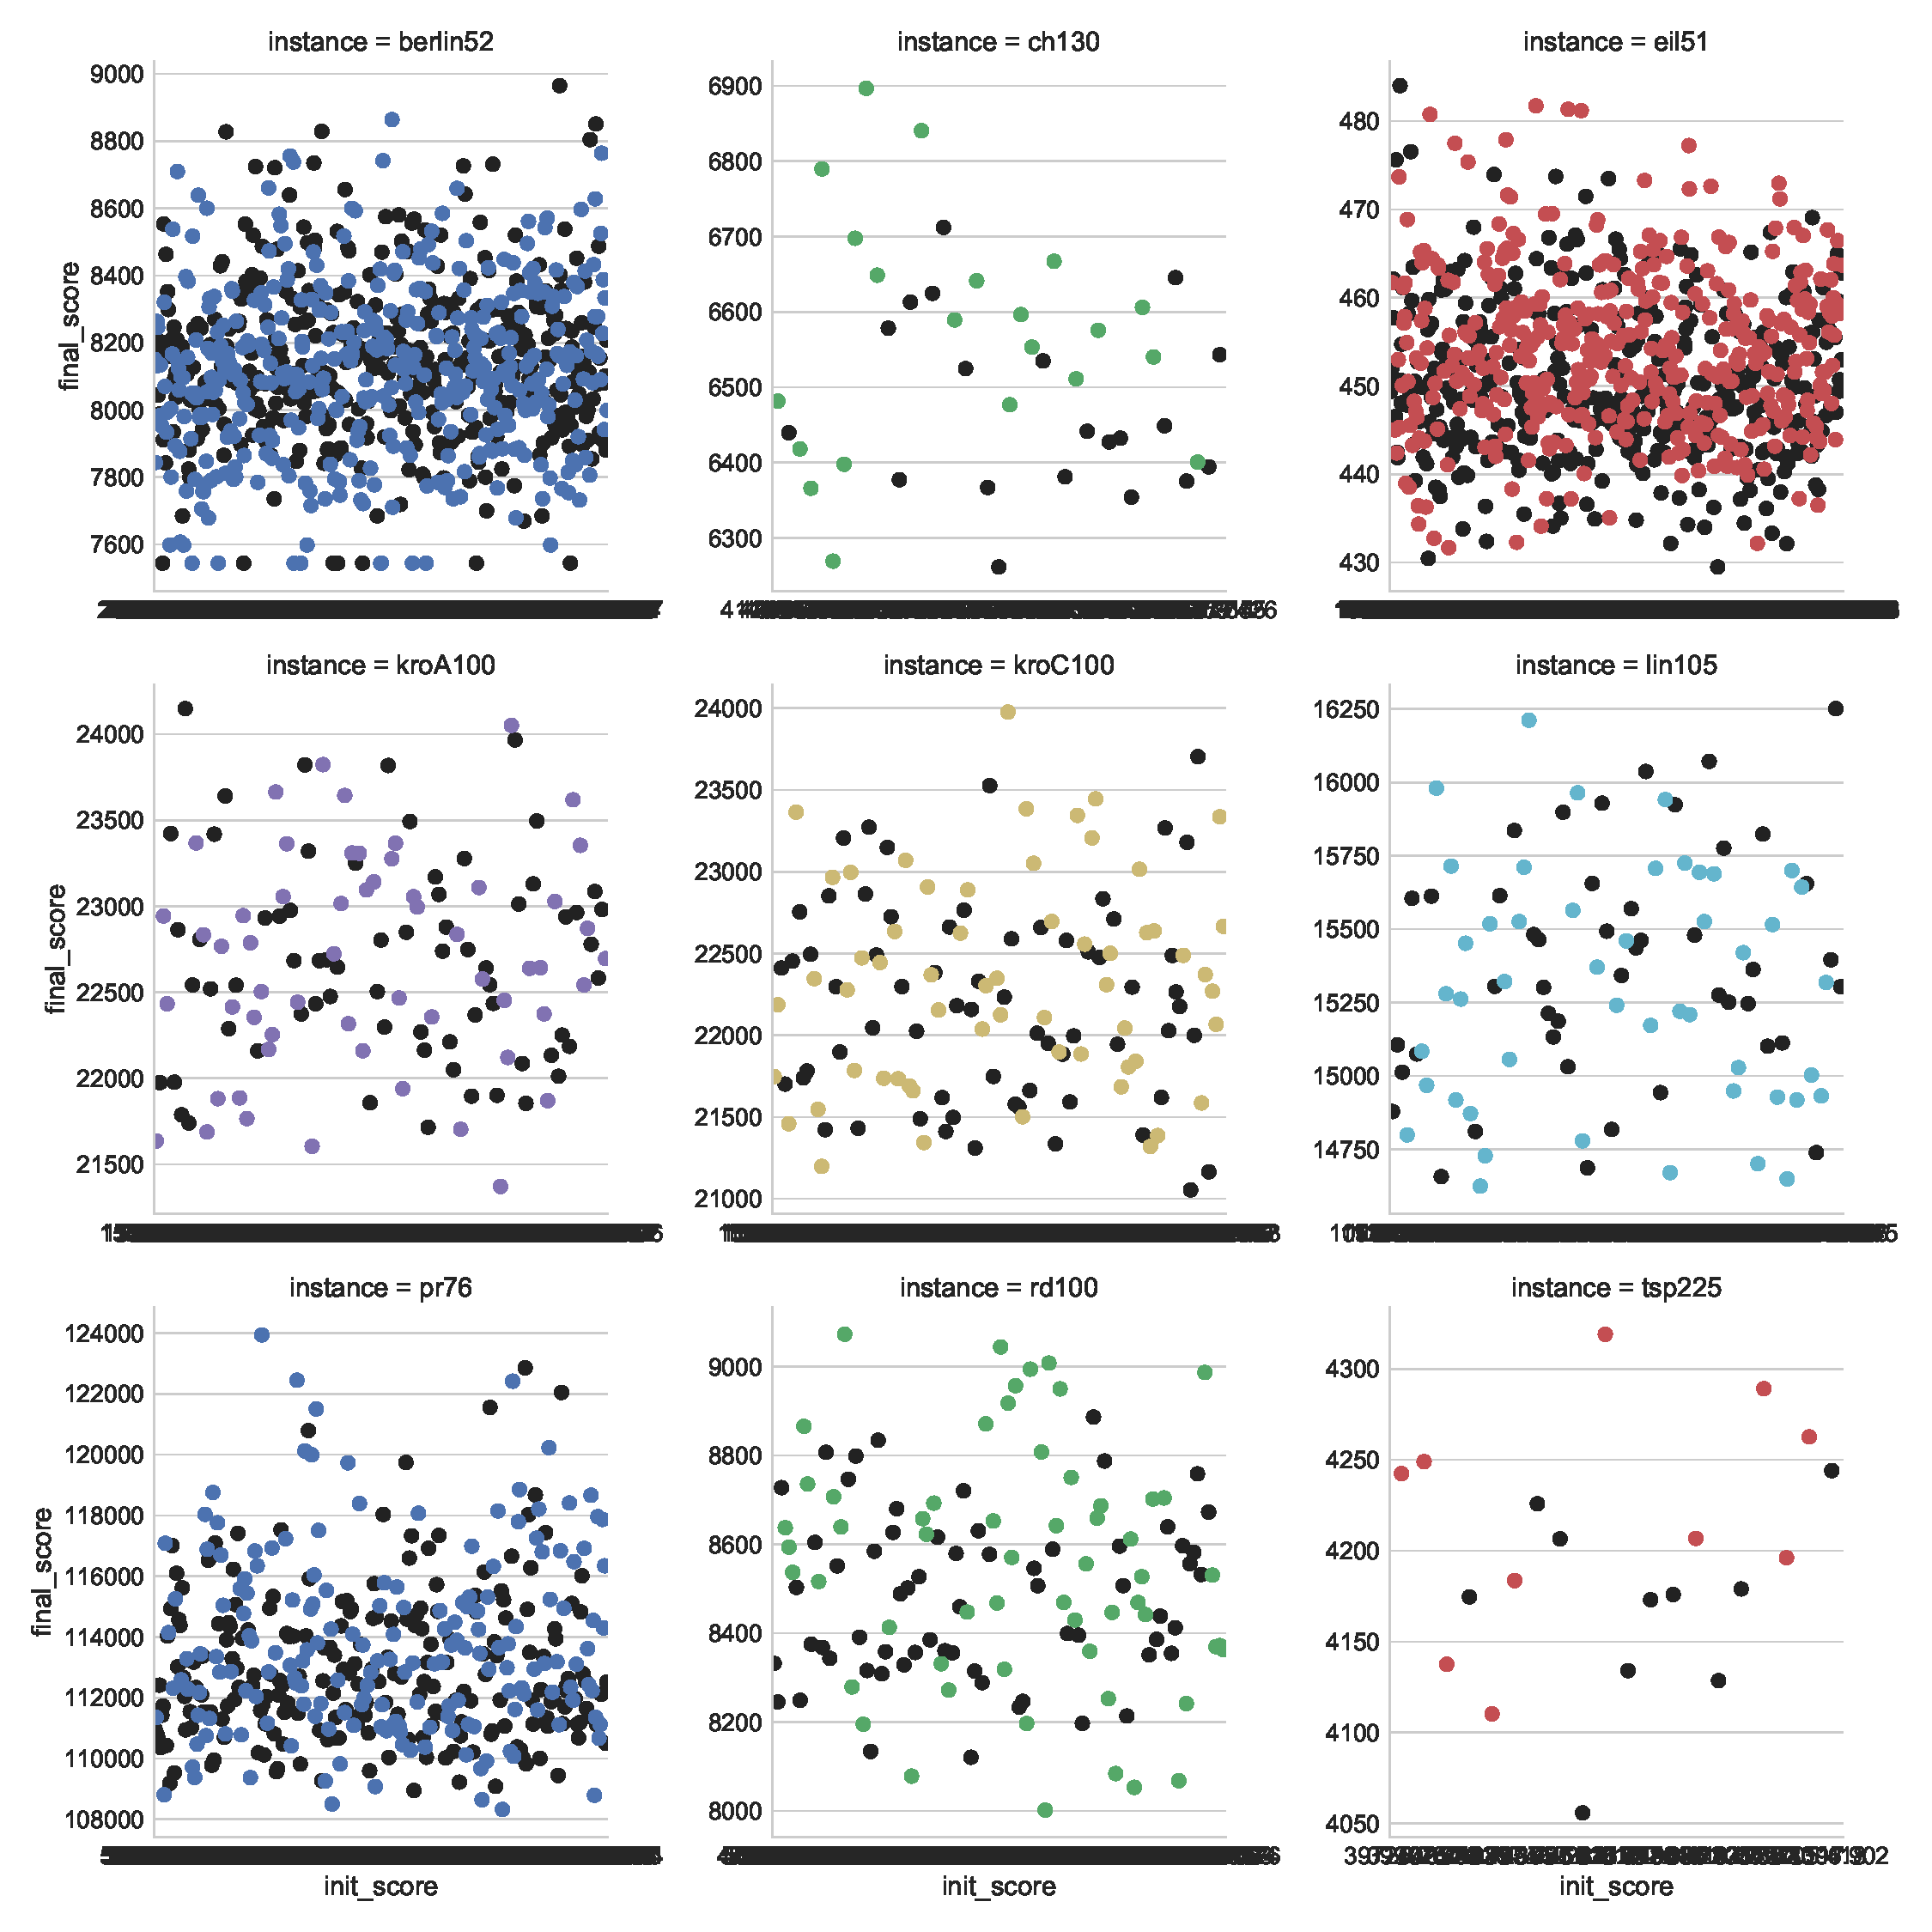
\includegraphics[width=1.0\textwidth]{graphs/init_vs_final_score_point.pdf}
\end{center}
\caption{Porównanie jakości rozwiązań początkowych i~końcowych przez~algorytmy Greedy (+) i~Steepest (x1) przedstawione na wykresie punktowym.}
\label{fig:diff_point}
\end{figure}

\begin{figure}[H]
\begin{center}
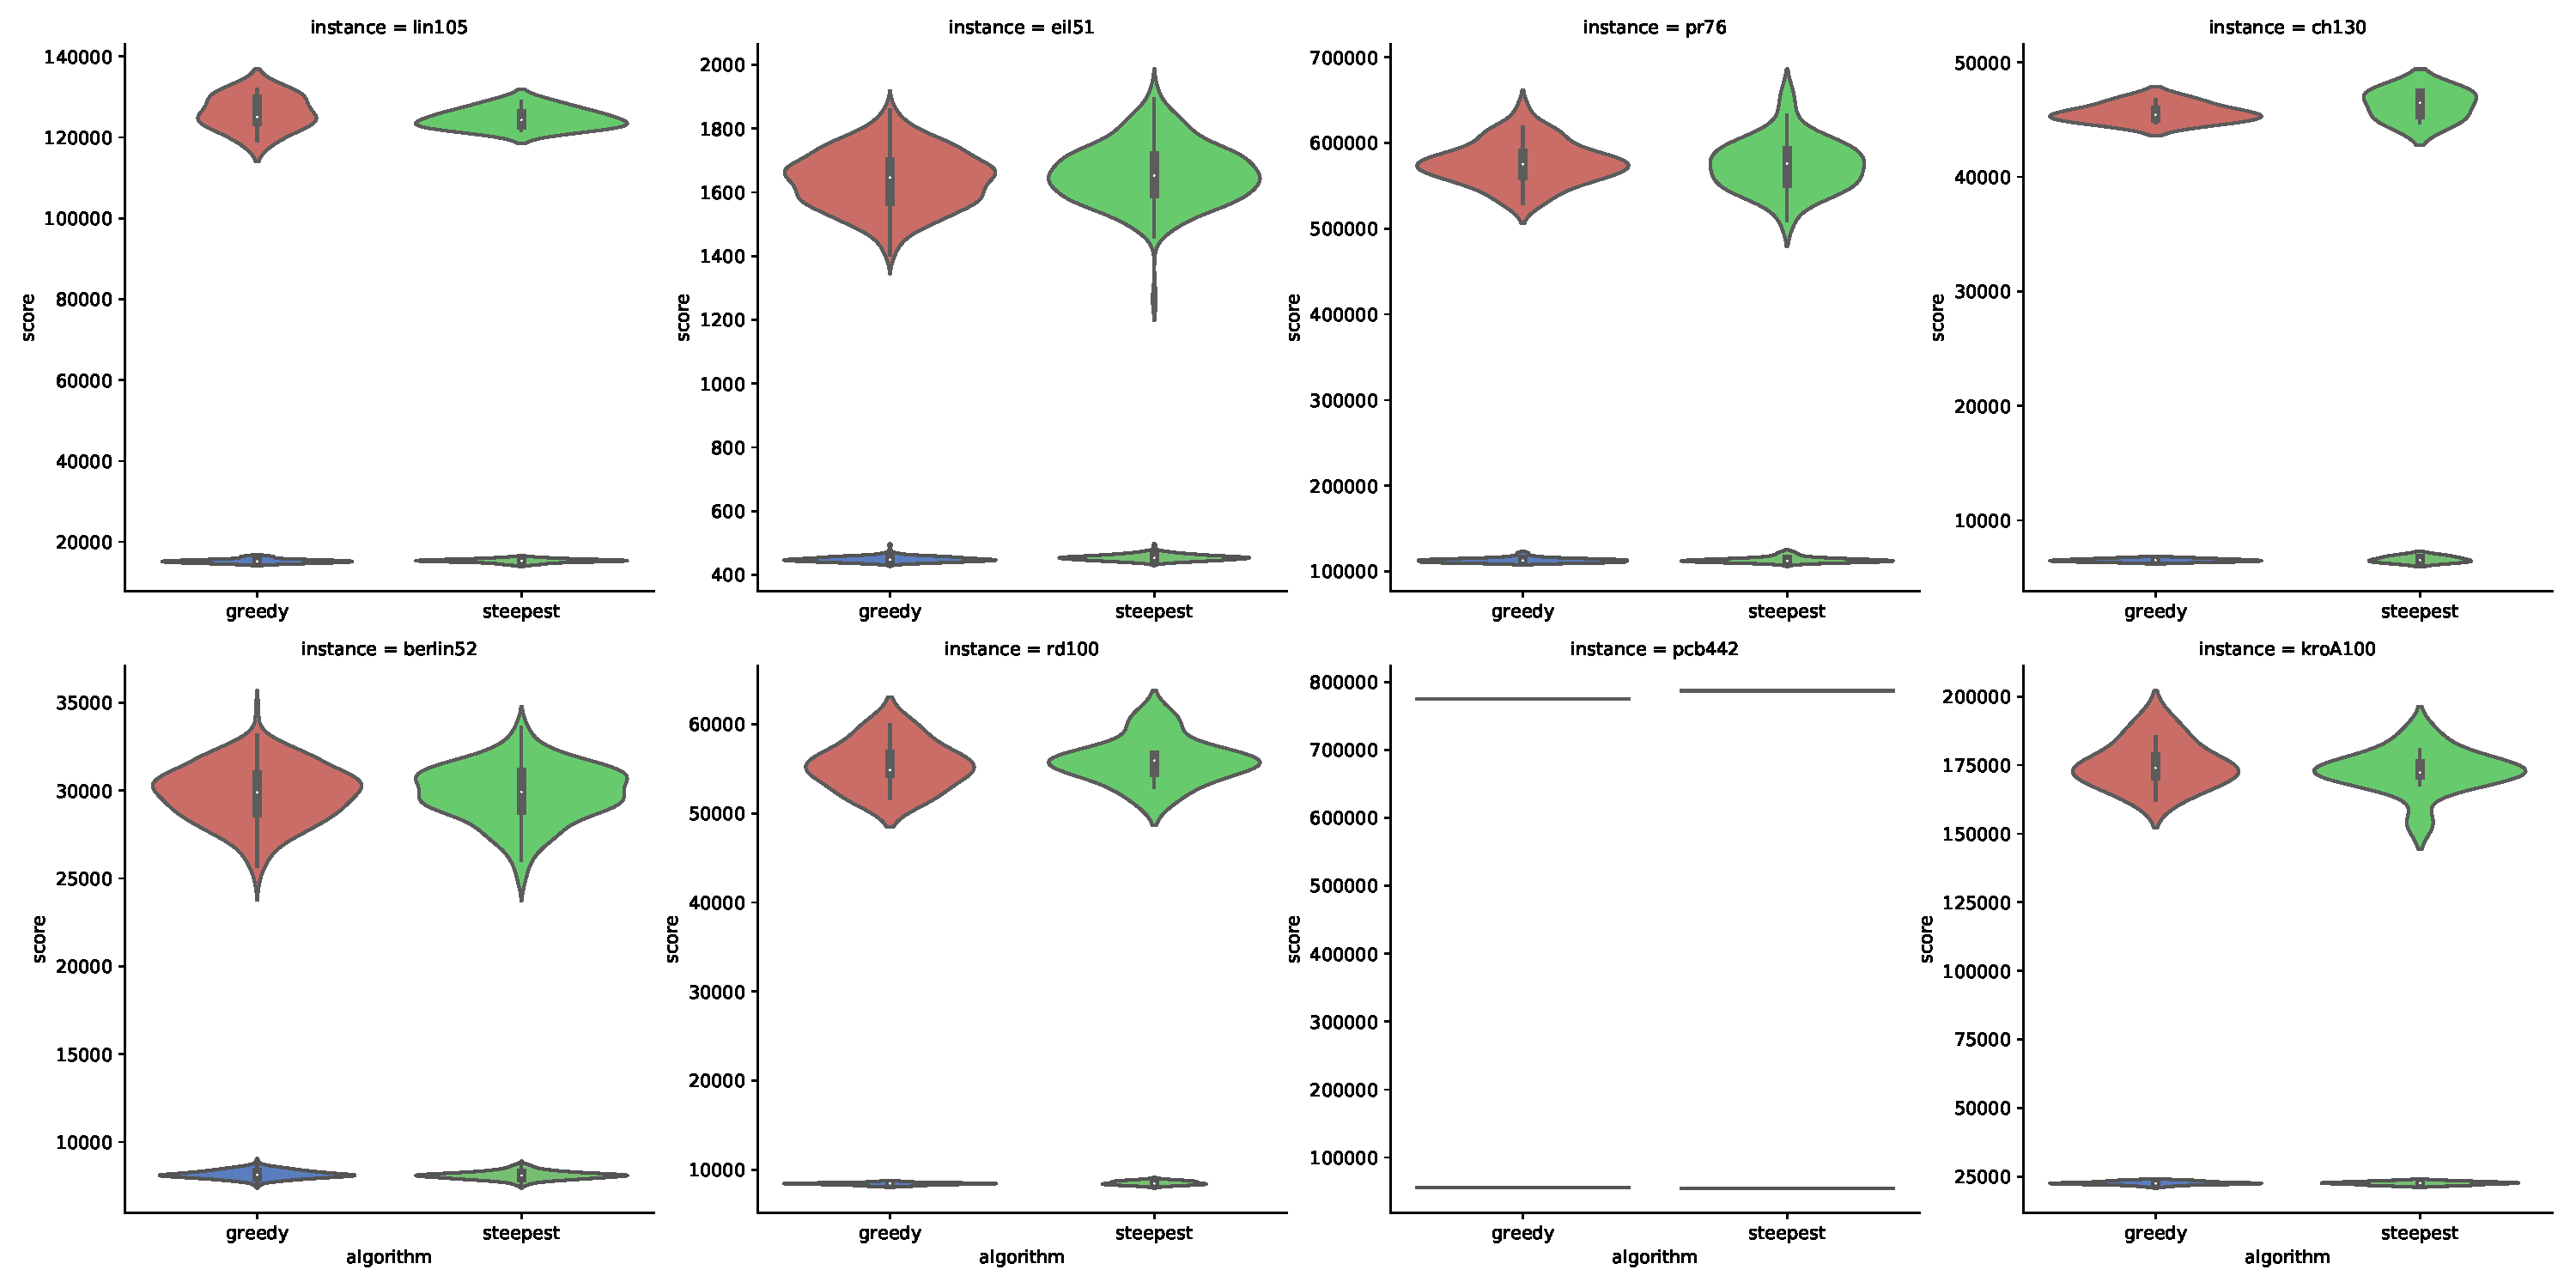
\includegraphics[width=1.0\textwidth]{graphs/init_vs_final_score_violin.pdf}
\end{center}
\caption{Porównanie jakości rozwiązań początkowych i~końcowych przez~algorytmy Greedy Search i~Steepest.}
\label{fig:diff}
\end{figure}

\subsubsection{Wielokrotne uruchamianie dla różnych rozwiązań początkowych}

Wykresy~\ref{fig:more_berlin} i~\ref{fig:more_eil} przedstawiają wartość najlepszego znalezionego rozwiązania po~i-tej iteracji. Jak~widać, poprawia się ona~co~pewien czas. Im~rozwiązanie jest lepsze, tym~ten~czas jest~dłuższy. Im~więcej razy algorytm będzie uruchamiany z~różnych rozwiązań początkowych, tym~istnieje większa szansa, że~osiągnie on~lepszy wynik, więc~warto powtarzać uruchomienia dla~różnych rozwiązań początkowych, aby~pełniej przeszukać przestrzeń wszystkich rozwiązań.

\begin{figure}[H]
\begin{center}
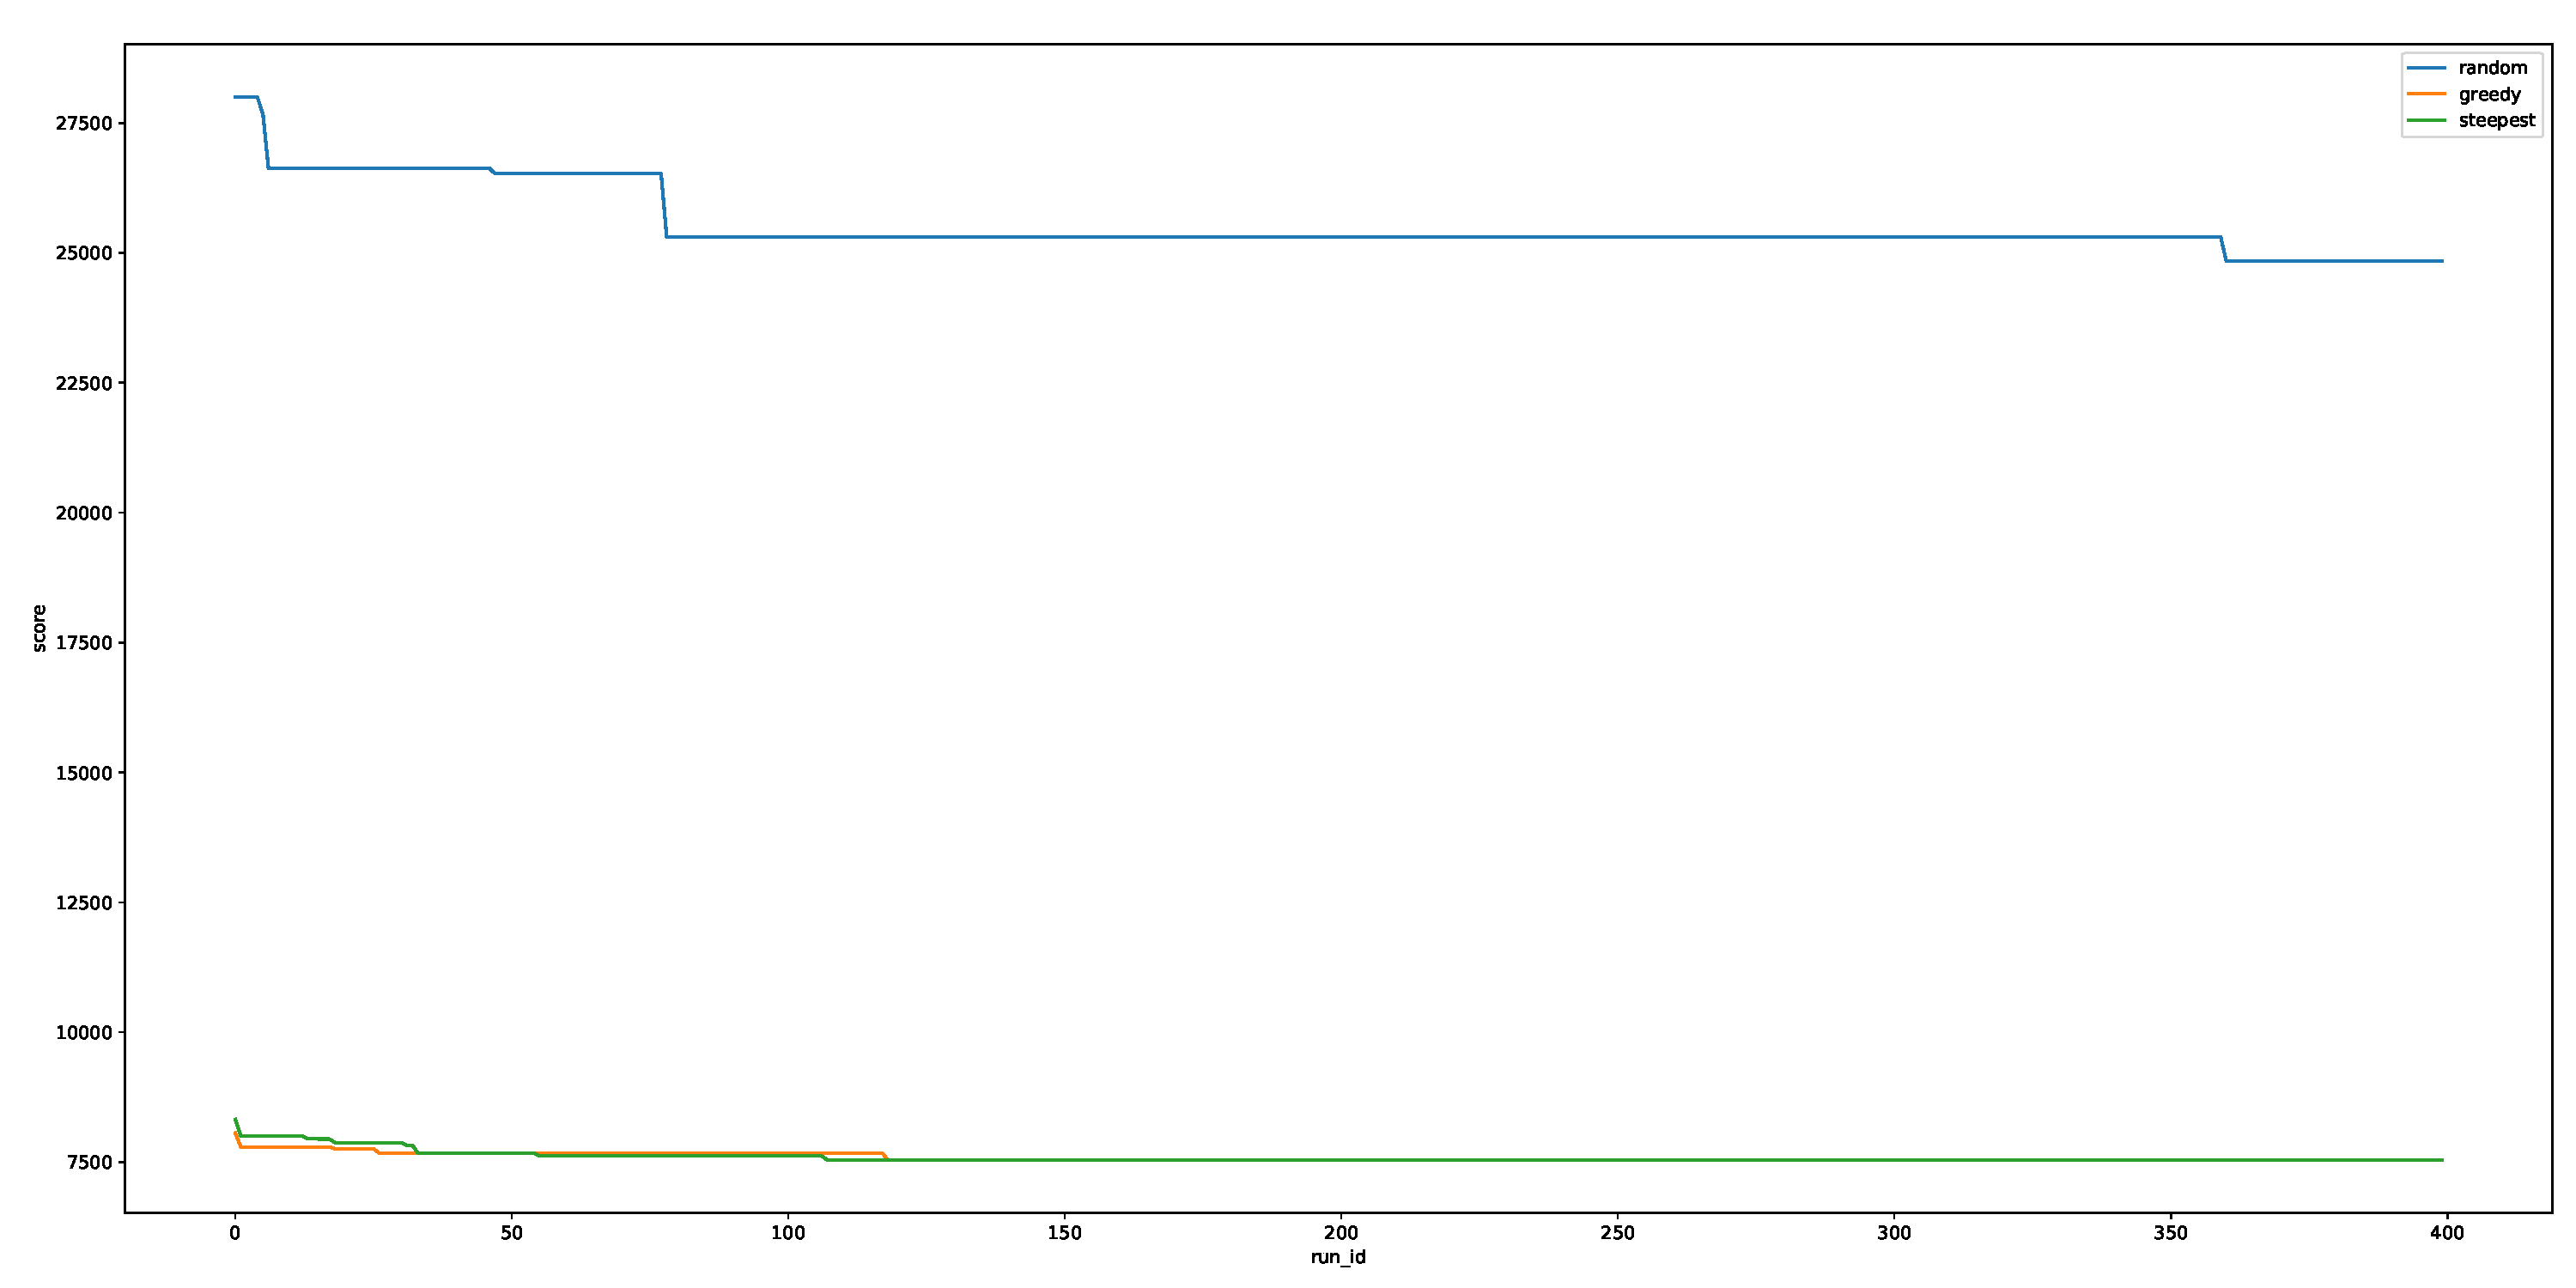
\includegraphics[width=1.0\textwidth]{graphs/multi_start_scoreberlin52.pdf}
\end{center}
\caption{Porównanie jakości rozwiązań algorytmów Gready Search i~Steepest w~zależności od~liczby uruchomień tych algorytmów dla~różnych rozwiązań początkowych dla~zbioru berlin52.}
\label{fig:more_berlin}
\end{figure}

\begin{figure}[H]
\begin{center}
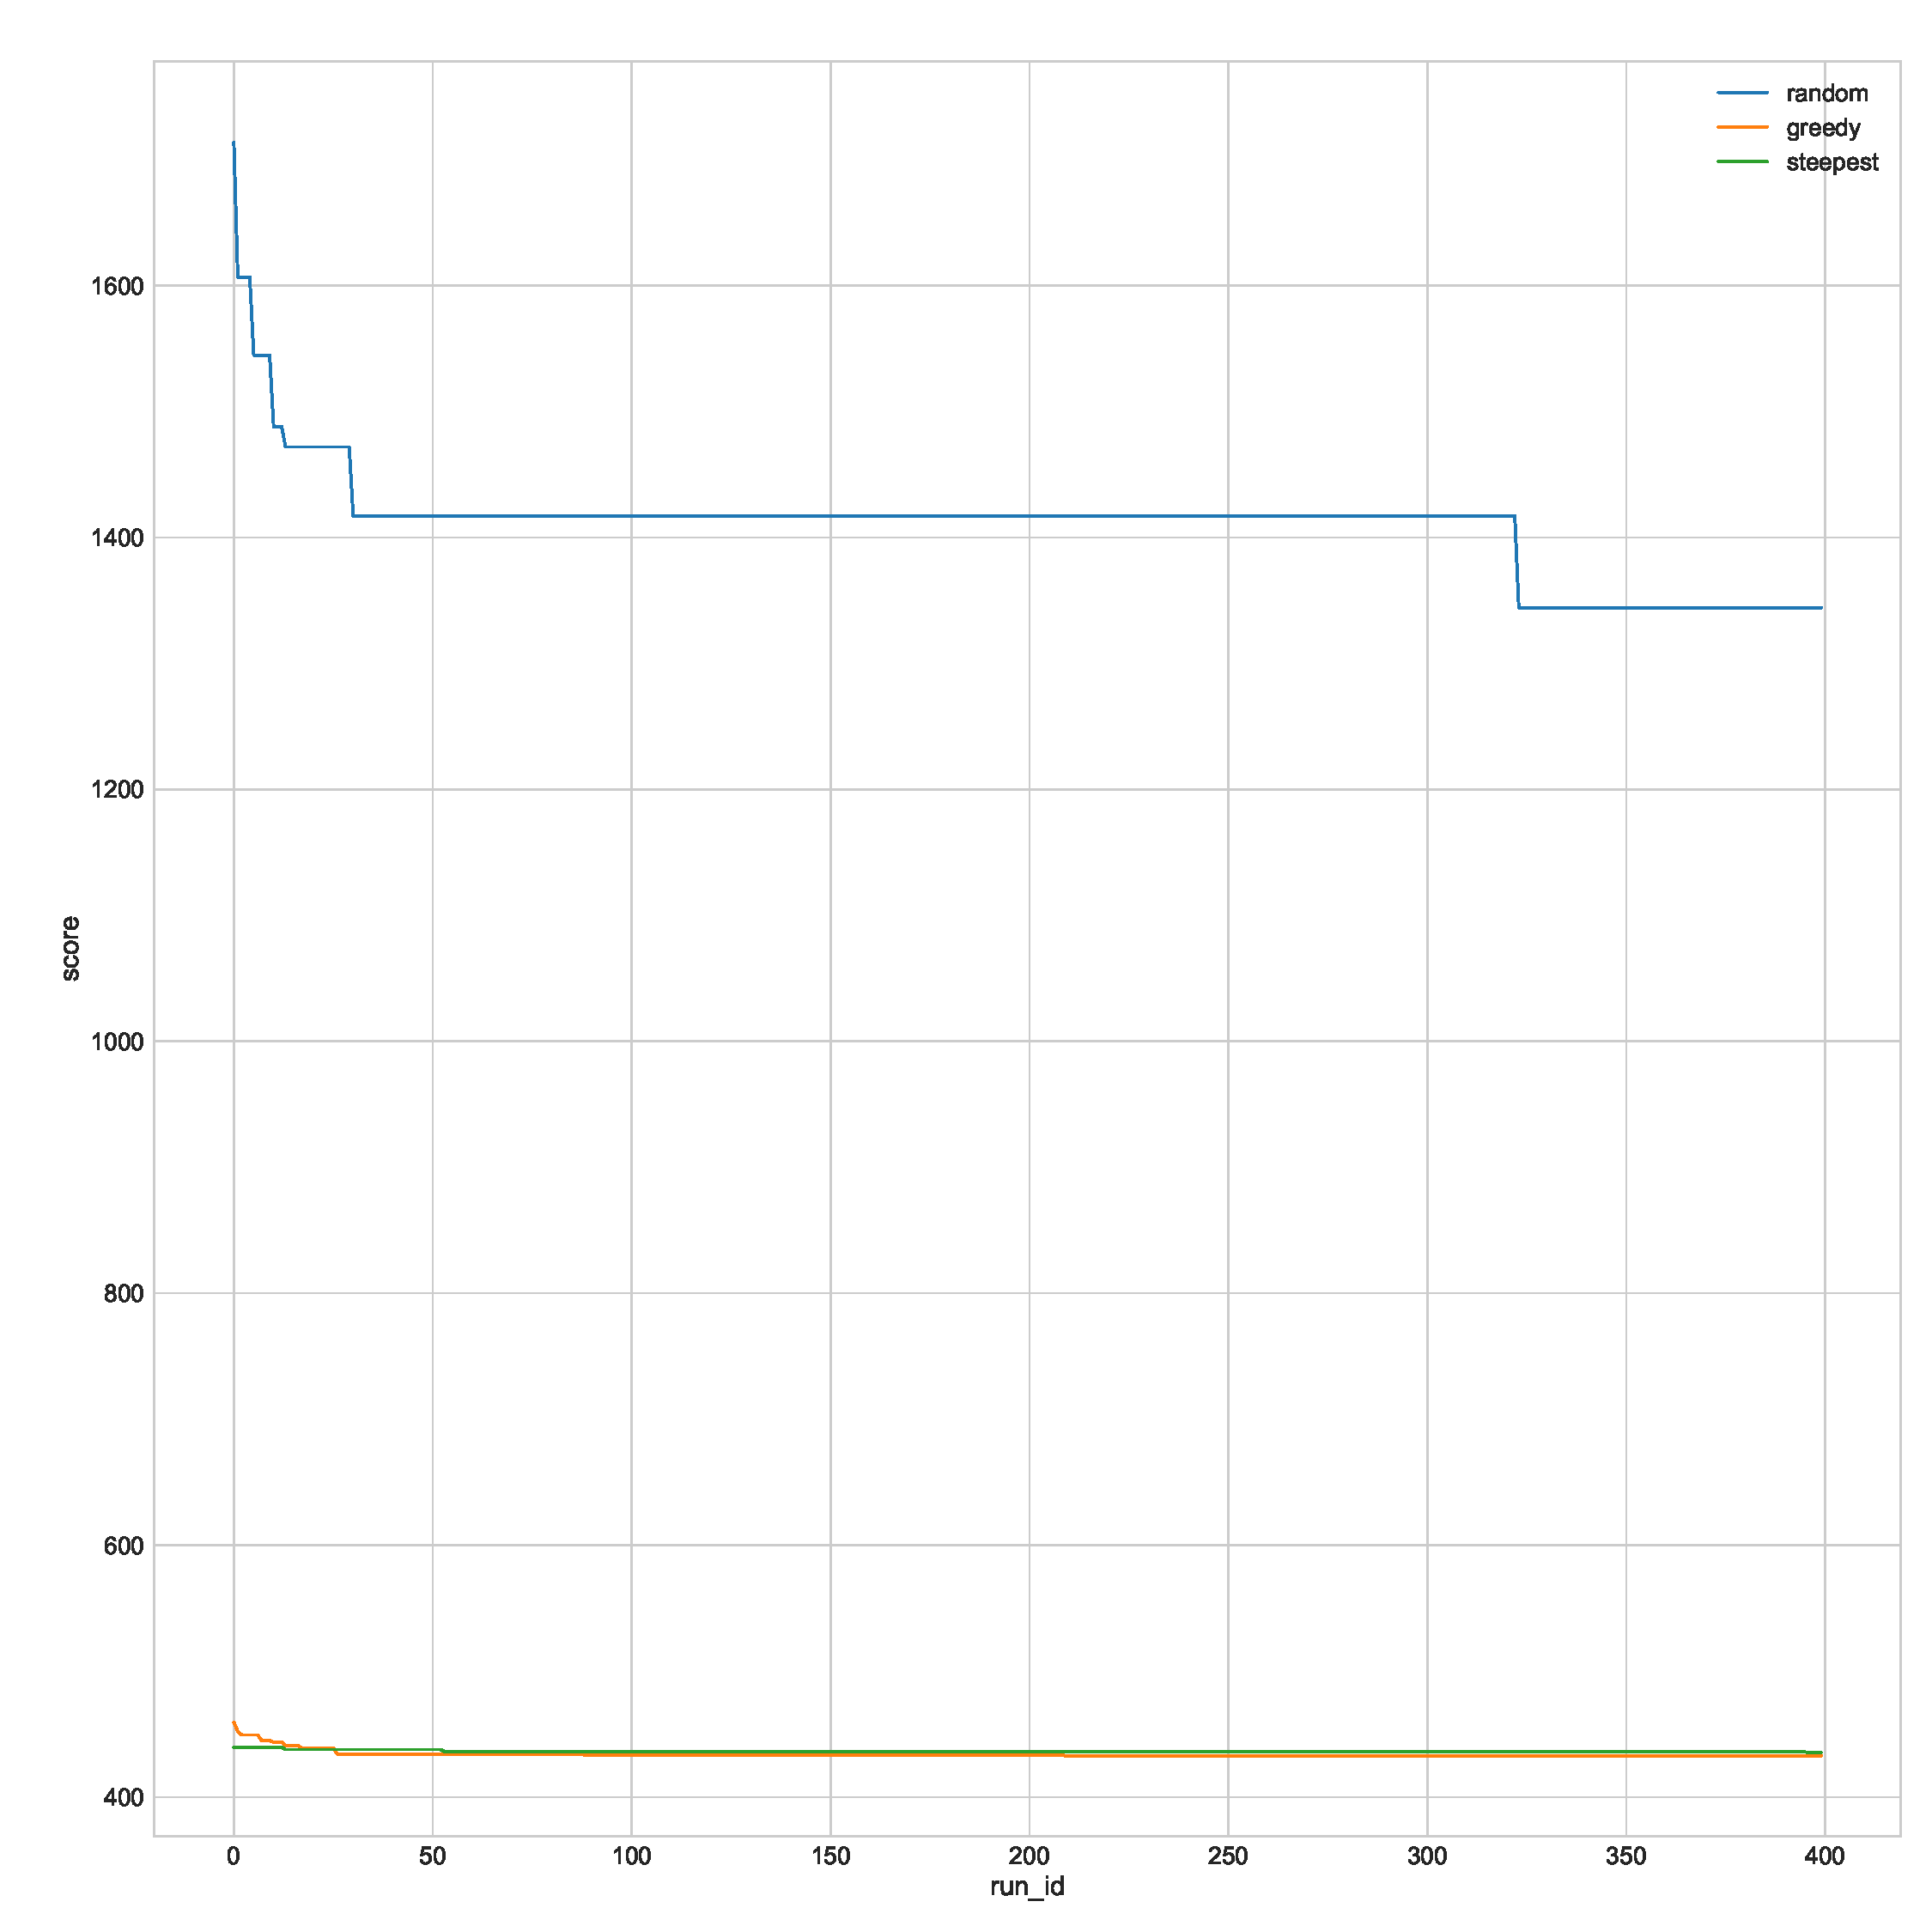
\includegraphics[width=1.0\textwidth]{graphs/multi_start_scoreeil51.pdf}
\end{center}
\caption{Porównanie jakości rozwiązań algorytmów Gready Search i~Steepest w~zależności od~liczby uruchomień tych algorytmów dla~różnych rozwiązań początkowych dla~zbioru eil51.}
\label{fig:more_eil}
\end{figure}

\subsection{Porównanie rozwiązań}

\subsubsection{Miara odległości rozwiązań od rozwiązania optymalnego}

Aby~porównywać między sobą rozwiązania, postanowiliśmy zbadać, jak~wiele mają takich samych krawędzi. Aby~to~zmierzyć, dla~każdej krawędzi w~jednym rozwiązaniu, sprawdzamy, czy~istnieje ona~w~drugim (skierowana w~dowolną stronę, ponieważ obie krawędzie są~symetryczne).

\subsubsection{Wyniki}

Na~rysunku~\ref{fig:sim} można zaobserwować podobieństwo rozwiązań znajdowanych przez algorytmy do~rozwiązania optymalnego. Istnieje wyraźna zależność polegająca na~tym, że~im~lepsze rozwiązanie, tym~jest~bardziej podobne do~optymalnego.

Bardzo mocno wyróżnia się chmura rozwiązań losowych -- jakość rozwiązań jest~bardzo różnorodna, ale~wszystkie są~bardzo mało podobne do~rozwiązania optymalnego (poniżej 10\%, a~im~więcej miast w~instancji, tym~mniej podobne).

\begin{figure}[H]
\begin{center}
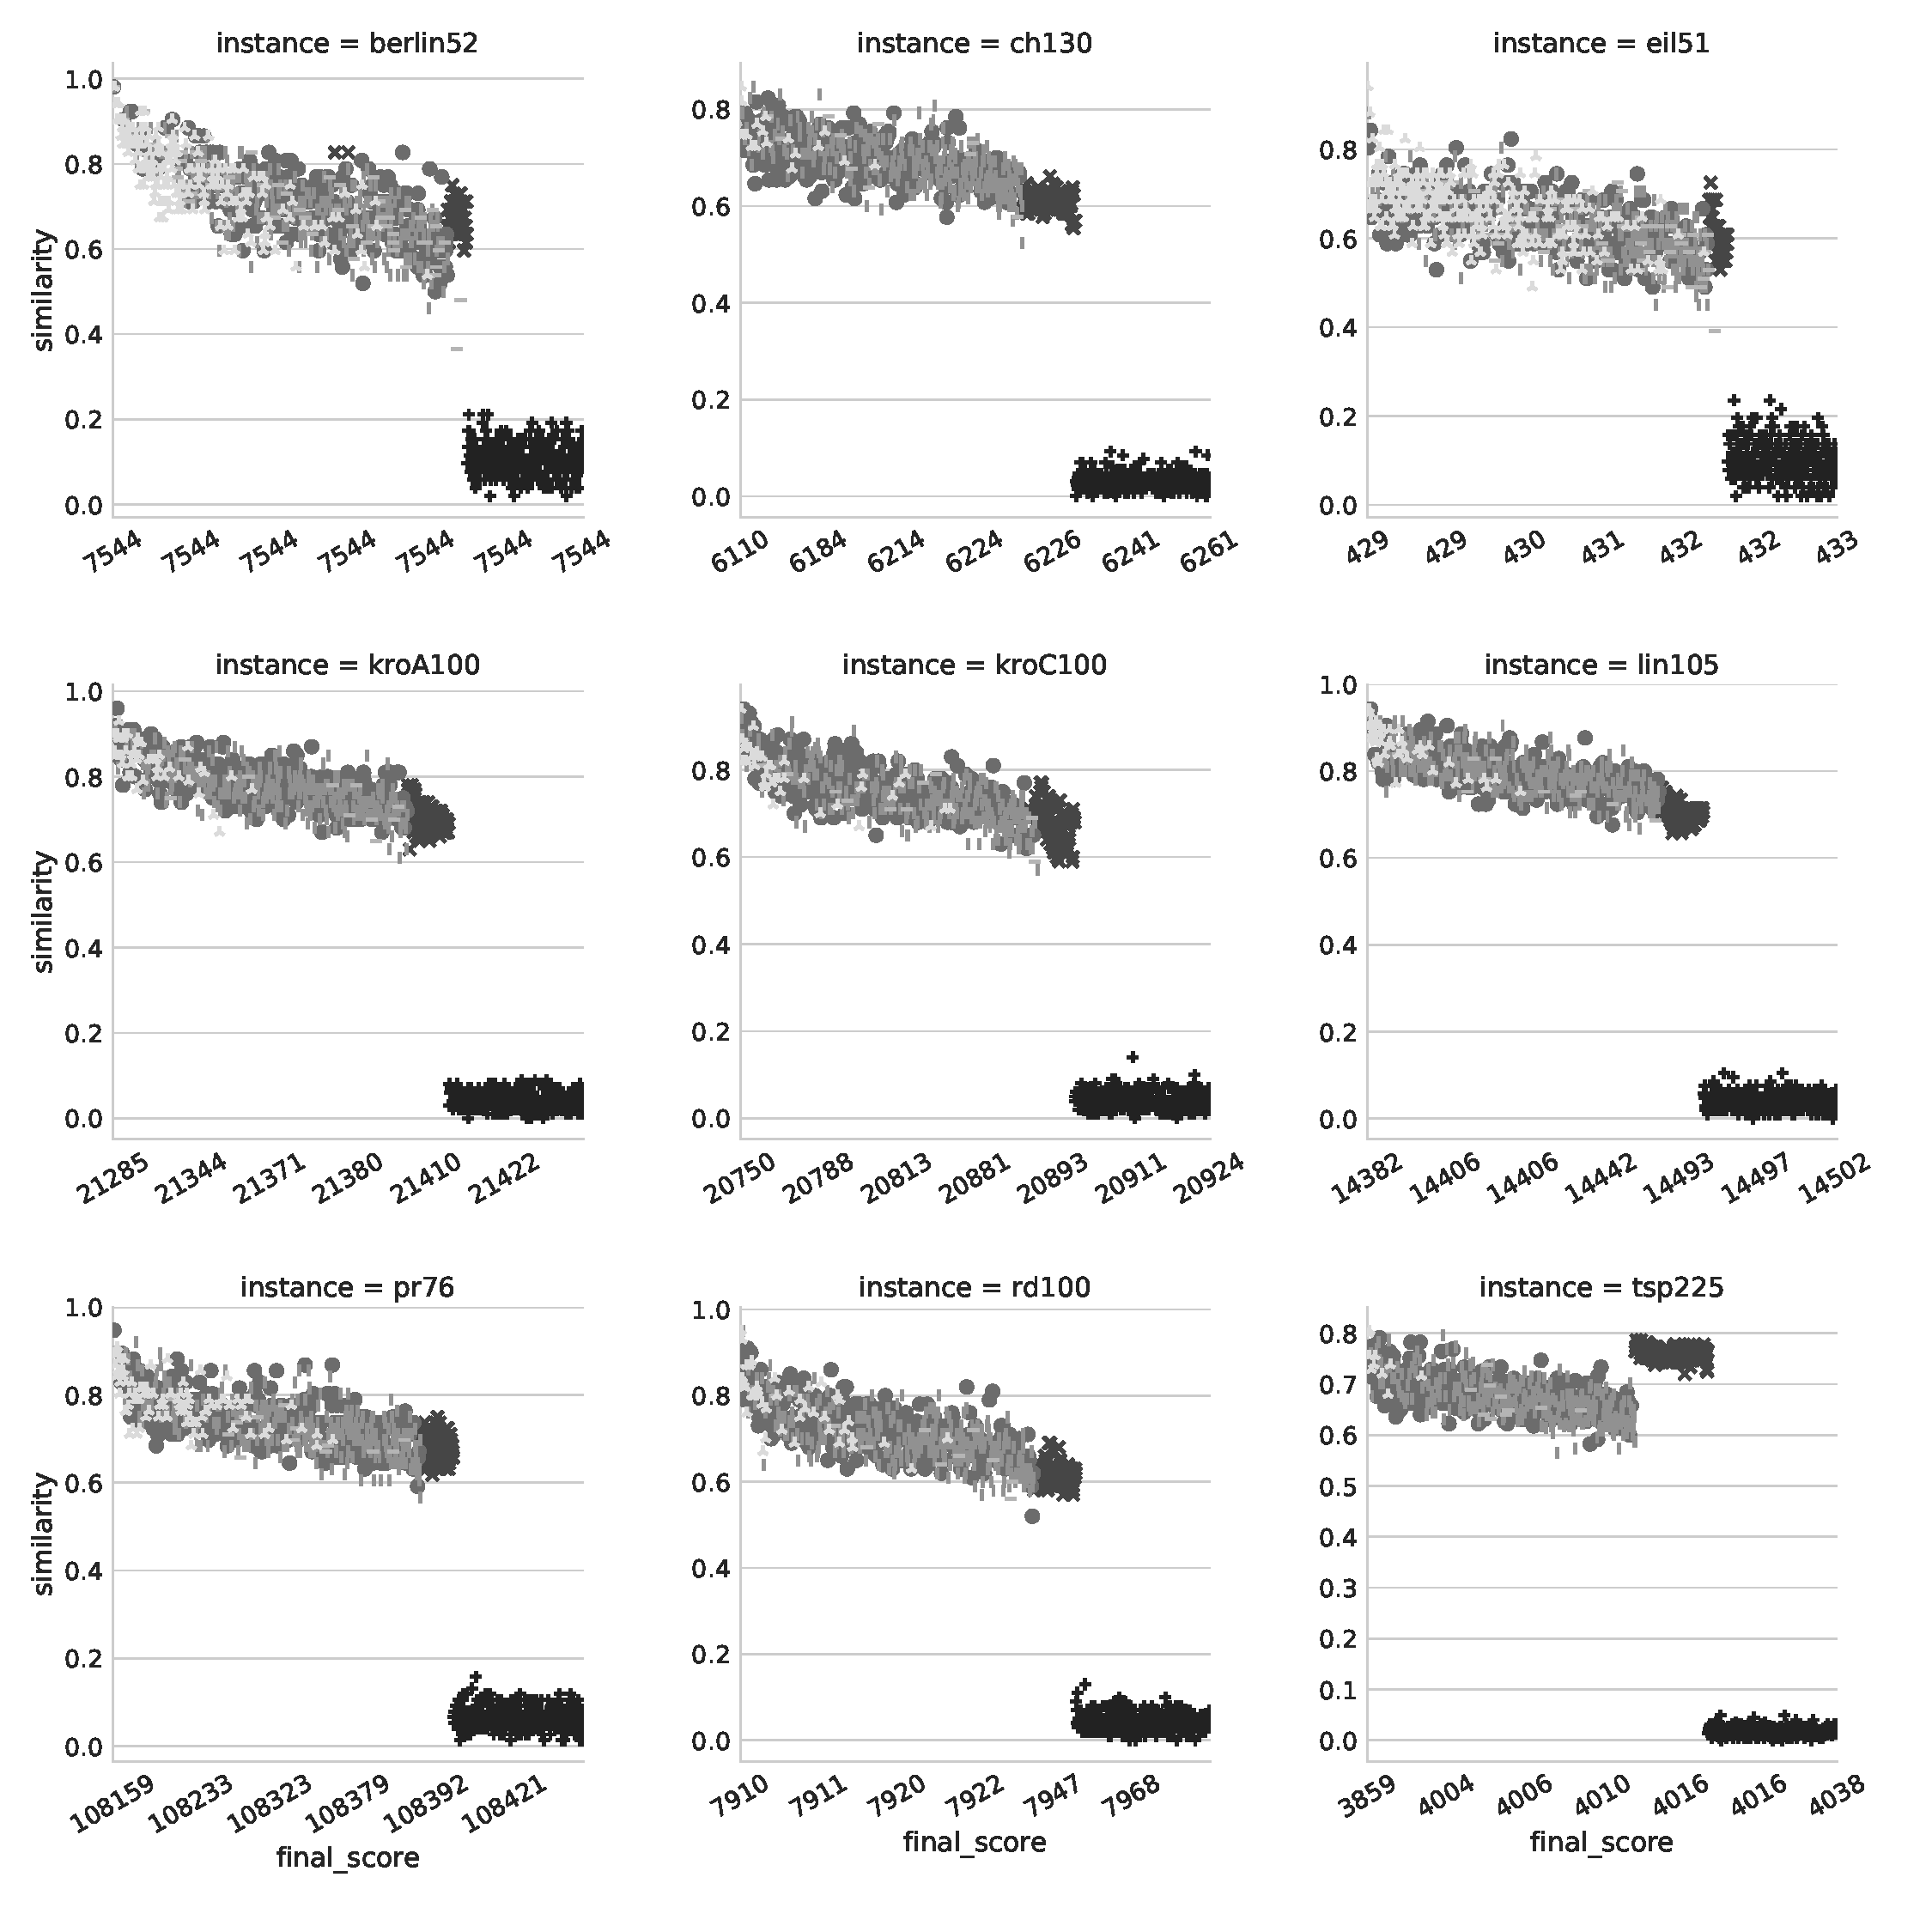
\includegraphics[width=1.0\textwidth]{graphs/similarity_comparision.pdf}
\end{center}
\caption{Porównanie odległości znajdowanych rozwiązań przez algorytmy od~rozwiązania optymalnego. Algorytm losowy (+), heurystyczny (x), Greedy (o), Steepest (I), TS (\_), SA (u)}.
\label{fig:sim}
\end{figure}